<<<<<<< HEAD
In this section, a comparison of instantaneous spanwise vorticity for the different meshes is shown in Figures \ref{fig:vorticity_Re200k_sp_210}, \ref{fig:vorticity_Re200k_sp_240},  \ref{fig:vorticity_Re200k_sp_270}, and \ref{fig:vorticity_Re200k_sp_300} for phases $\psi=210^\circ$, $\psi=240^\circ$, $\psi=270^\circ$, and $\psi=300^\circ$ respectively. 

For $\psi=210^\circ$, for $Re=200,000$, flow is still attached to the airfoil. 
Note that for $Re=40,000$ for the same advance ratio (see Figure \ref{fig:vorticity_zonal_210}), vorticity roll-up and LEV formation is seen at this phase.
M0\_nz50 mesh shows poor resolution in the wake of the airfoil.
Mza1\_nz50 and Mza1\_nz100 show a similar resolution of the wake, with some diffused flow structures resolved.
Mza2\_nz50, which is the finest mesh considered here, shows the best resolution. 

For $\psi=240^\circ$, formation of LEV is seen for all meshes.
Note that as compared to $Re=40,000$ case, LEV forms closer to the leading edge.
LEV for M0\_nz50 is diffused compared to other finer meshes, along with poor resolution of flow structures over the airfoil surface.
Mza1\_nz50, Mza1\_nz100, and Mza2\_nz50 meshes compare well, with Mza2\_nz50 showing the best resolution.


At $\psi=270^\circ$, LEV has ejected from the airfoil surface. 
Formation of TEV can also be seen at this phase.
For M0\_nz50 mesh, the LEV, the shear layer leading up to the LEV, and the TEV all show poor resolution.
LEV and shear layer is best resolved for Mza2\_nz50 mesh.
TEV resolution is similar between Mza1\_nz50 and Mza2\_nz50 meshes.


At $\psi=300^\circ$, LEV advects further away from the airfoil. A larger TEV is also seen at this phase.
LEV resolution is best for Mza2\_nz50 mesh, and worst for M0\_nz50 mesh. 
TEV and shear layer resolution near the airfoil surface compare well between Mza1\_nz50 and Mza2\_nz50 meshes.


A more quantitive comparison of the LEV including tangential velocity profiles and LEV location for different phases in the surging cycle is mentioned in the following sections.


%%=====================================
%% Phase = 210
%%=====================================

\begin{figure}[H]
	\centering
	\begin{center}
		\begin{subfigure}[b]{0.6\textwidth}
			\centering
			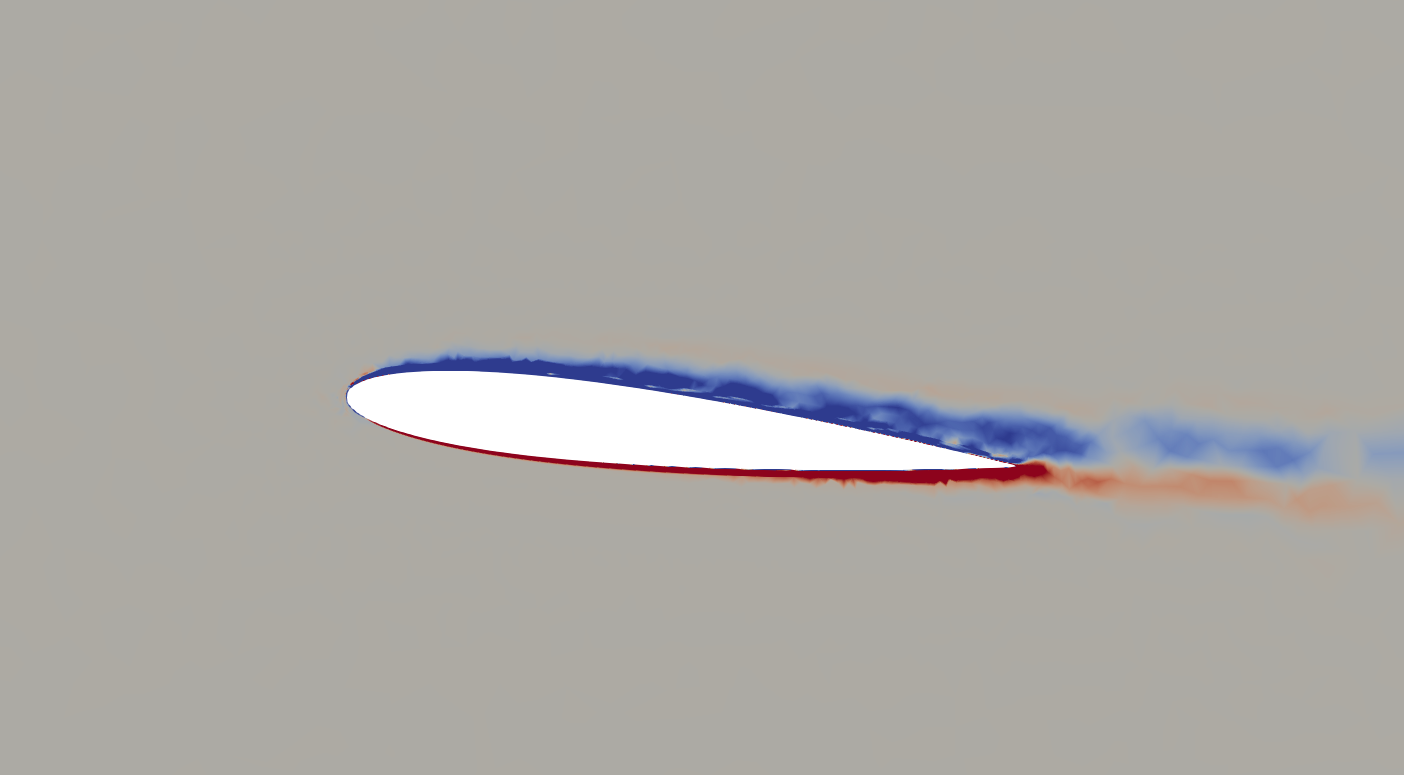
\includegraphics[width=1\textwidth]{figures/zonal_adapt_results/vorticity_plots_Re200k/M0/phase_210.png}
			\caption{M0\_nz50 mesh, $\psi$ = $210^\circ$}
			\label{fig:M0_Re200k_sp_psi210}
		\end{subfigure}
	\end{center}

	\begin{subfigure}[b]{0.6\textwidth}
		\centering
		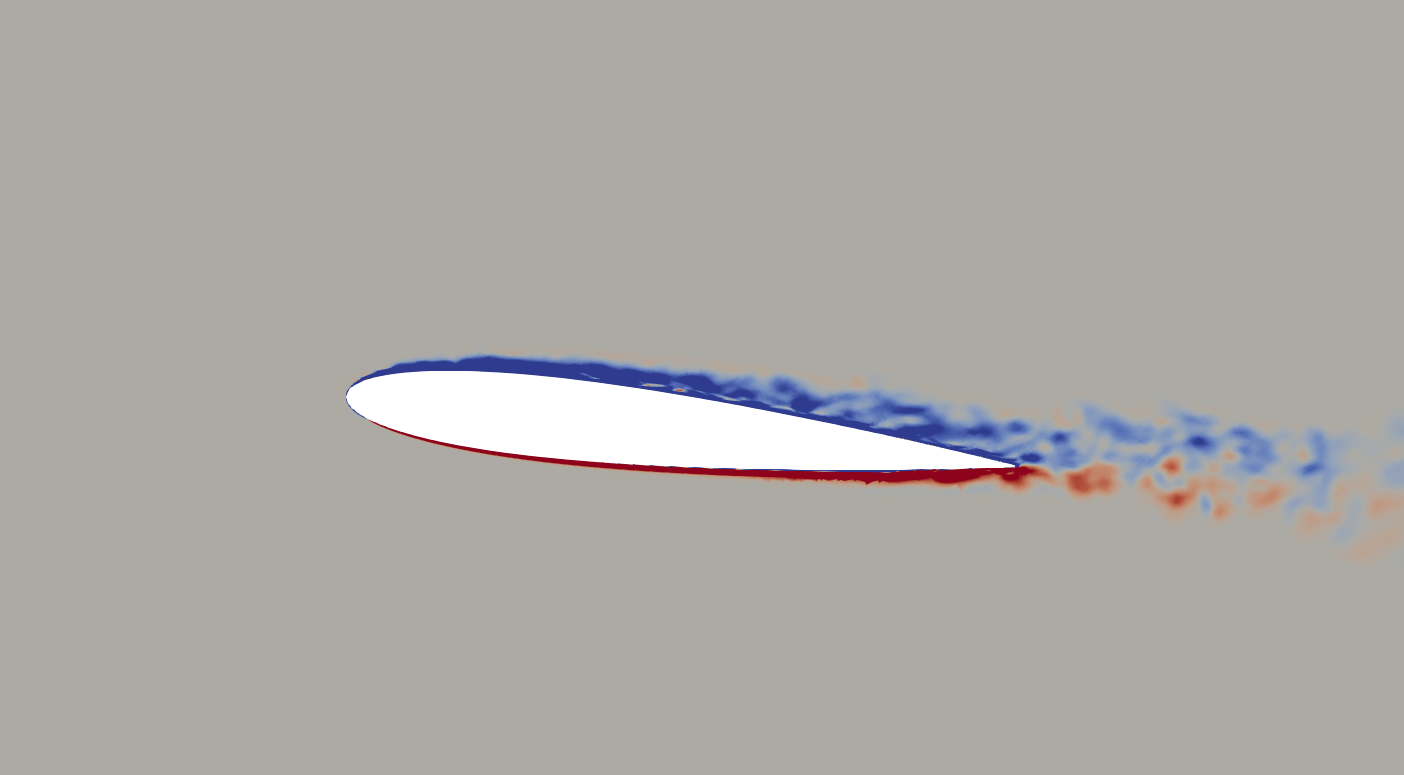
\includegraphics[width=1\textwidth]{figures/zonal_adapt_results/vorticity_plots_Re200k/Mza1_50/phase_210.png}
		\caption{Mza1\_nz05 mesh, $\psi$ = $210^\circ$}
		\label{fig:Mza1_50_Re200k_sp_psi210}
	\end{subfigure}
%	\begin{subfigure}[b]{0.475\textwidth}
%		\centering
%		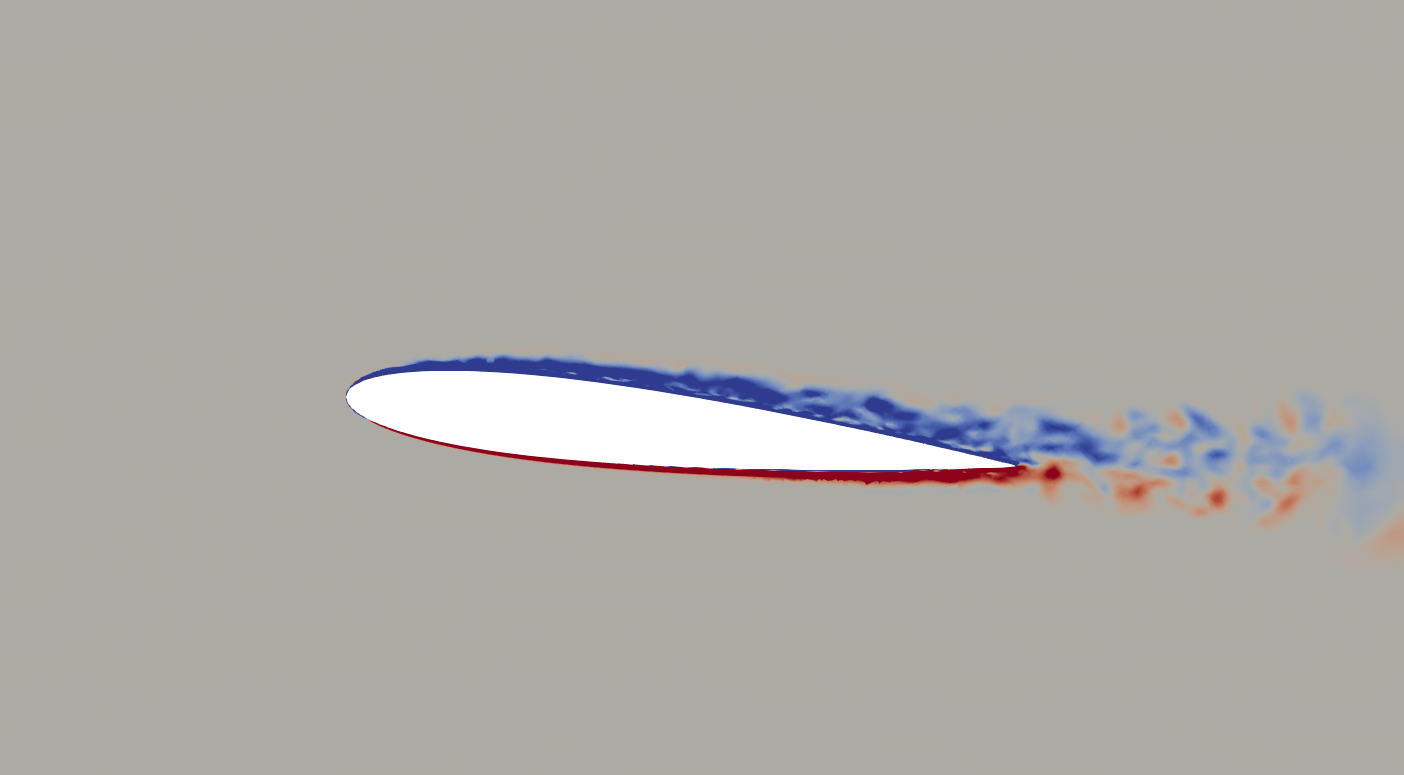
\includegraphics[width=1\textwidth]{figures/zonal_adapt_results/vorticity_plots_Re200k/Mza1_100/phase_210.png}
%		\caption{Mza1\_100 mesh, $\psi$ = $210^\circ$}
%		\label{fig:Mza1_100_Re200k_sp_psi210}
%	\end{subfigure}
	\begin{subfigure}[b]{0.6\textwidth}
		\centering
		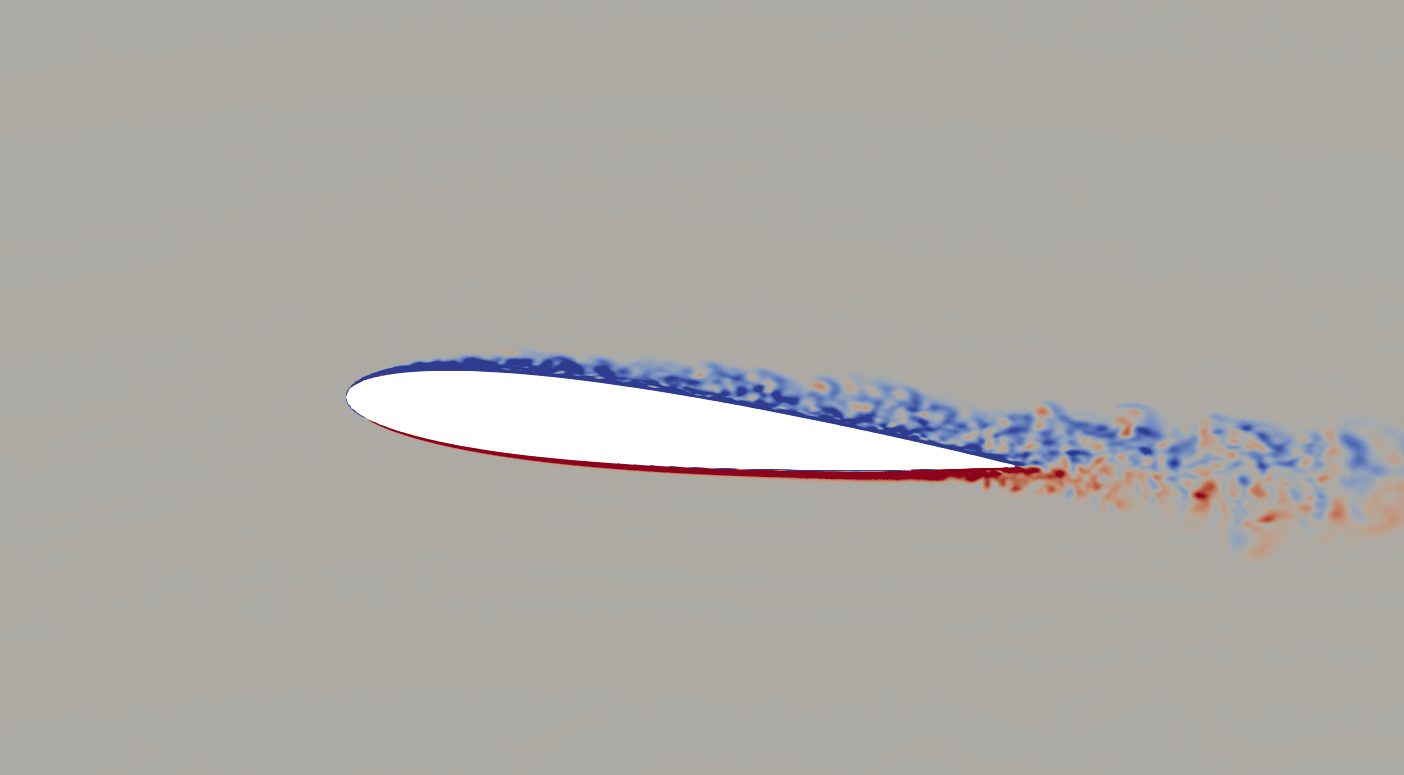
\includegraphics[width=1\textwidth]{figures/zonal_adapt_results/vorticity_plots_Re200k/Mza2_50/phase_210.png}
		\caption{Mza2\_nz50 mesh, $\psi$ = $210^\circ$}
		\label{fig:Mza2_50_Re200k_sp_psi210}
	\end{subfigure}	
	\caption{Spanwise vorticity comparison at $\psi$ = $210^\circ$ for different meshes}
	\label{fig:vorticity_Re200k_sp_210}
\end{figure}



%%=====================================
%% Phase = 240
%%=====================================


\begin{figure}[H]
	\centering
	\begin{center}
		\begin{subfigure}[b]{0.6\textwidth}
			\centering
			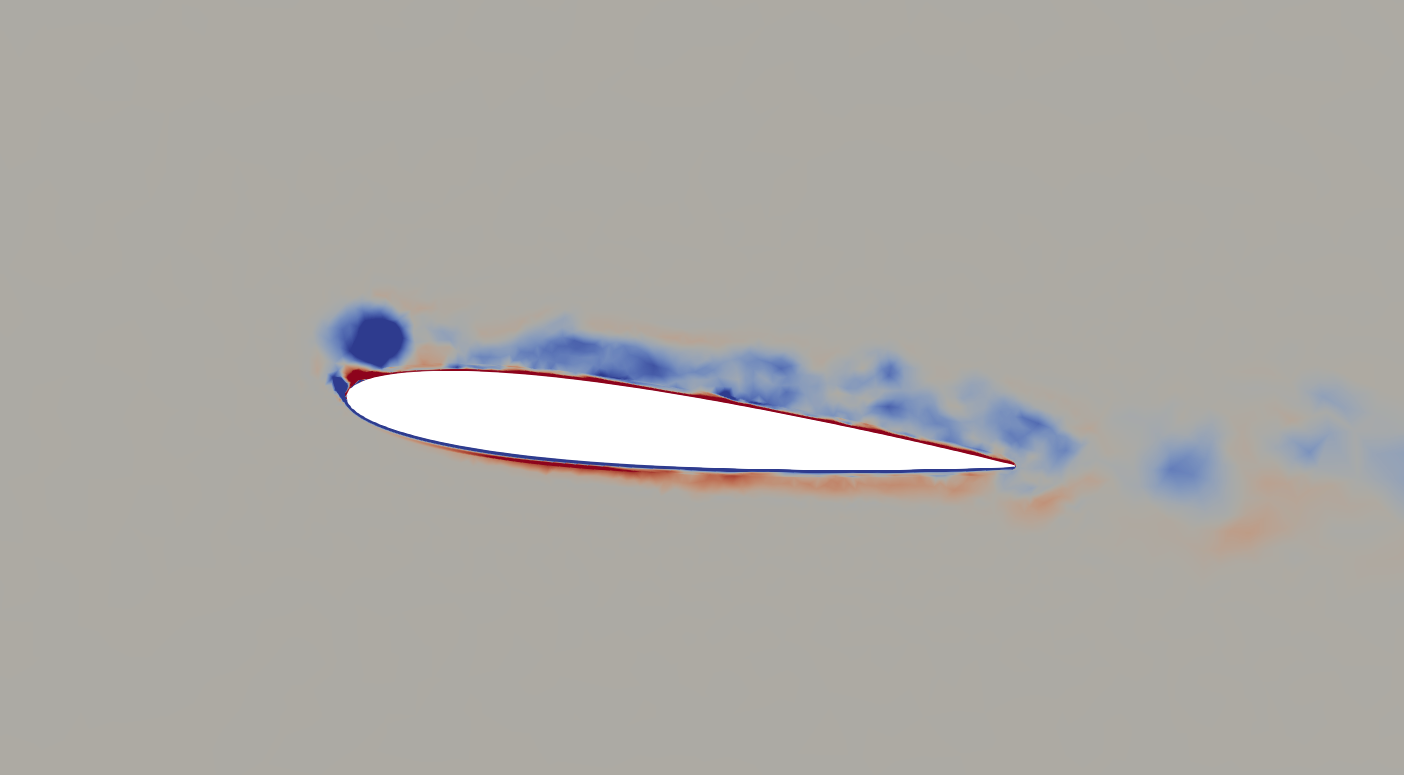
\includegraphics[width=1\textwidth]{figures/zonal_adapt_results/vorticity_plots_Re200k/M0/phase_240.png}
			\caption{M0\_nz50 mesh, $\psi$ = $240^\circ$}
			\label{fig:M0_Re200k_sp_psi240}
		\end{subfigure}
	\end{center}
	\begin{subfigure}[b]{0.6\textwidth}
		\centering
		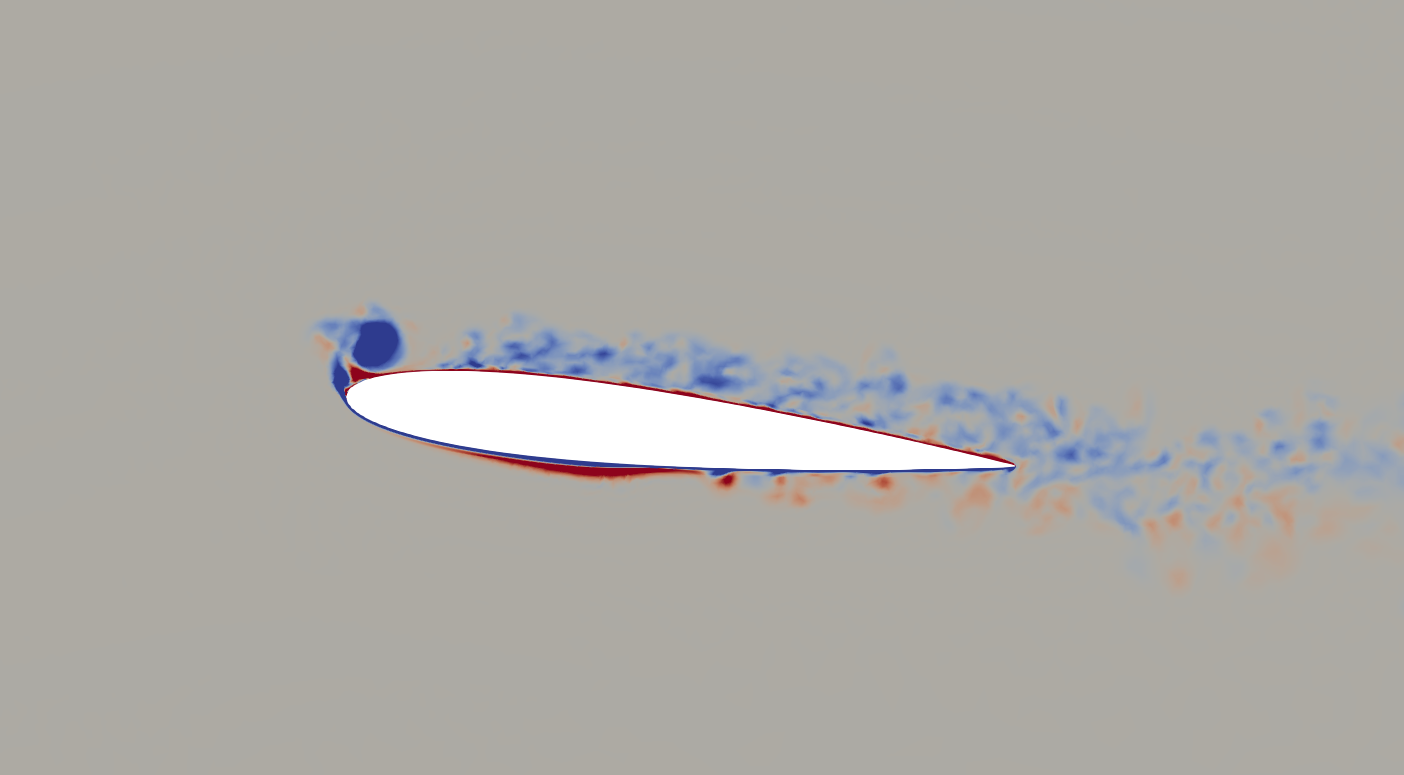
\includegraphics[width=1\textwidth]{figures/zonal_adapt_results/vorticity_plots_Re200k/Mza1_50/phase_240.png}
		\caption{Mza1\_nz50 mesh, $\psi$ = $240^\circ$}
		\label{fig:Mza1_50_Re200k_sp_psi240}
	\end{subfigure}
%	\begin{subfigure}[b]{0.475\textwidth}
%		\centering
%		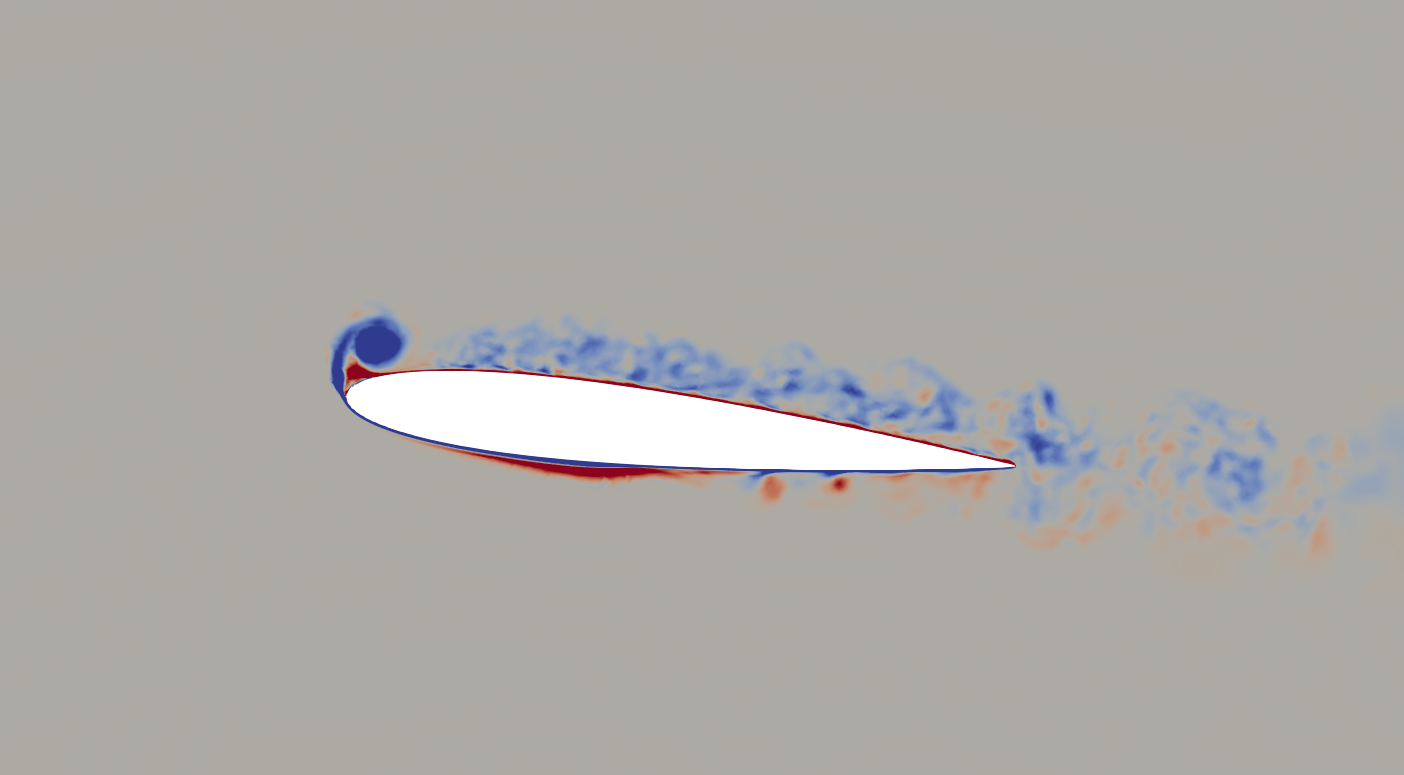
\includegraphics[width=1\textwidth]{figures/zonal_adapt_results/vorticity_plots_Re200k/Mza1_100/phase_240.png}
%		\caption{Mza1\_100 mesh, $\psi$ = $240^\circ$}
%		\label{fig:Mza1_100_Re200k_sp_psi240}
%	\end{subfigure}
	\begin{subfigure}[b]{0.6\textwidth}
		\centering
		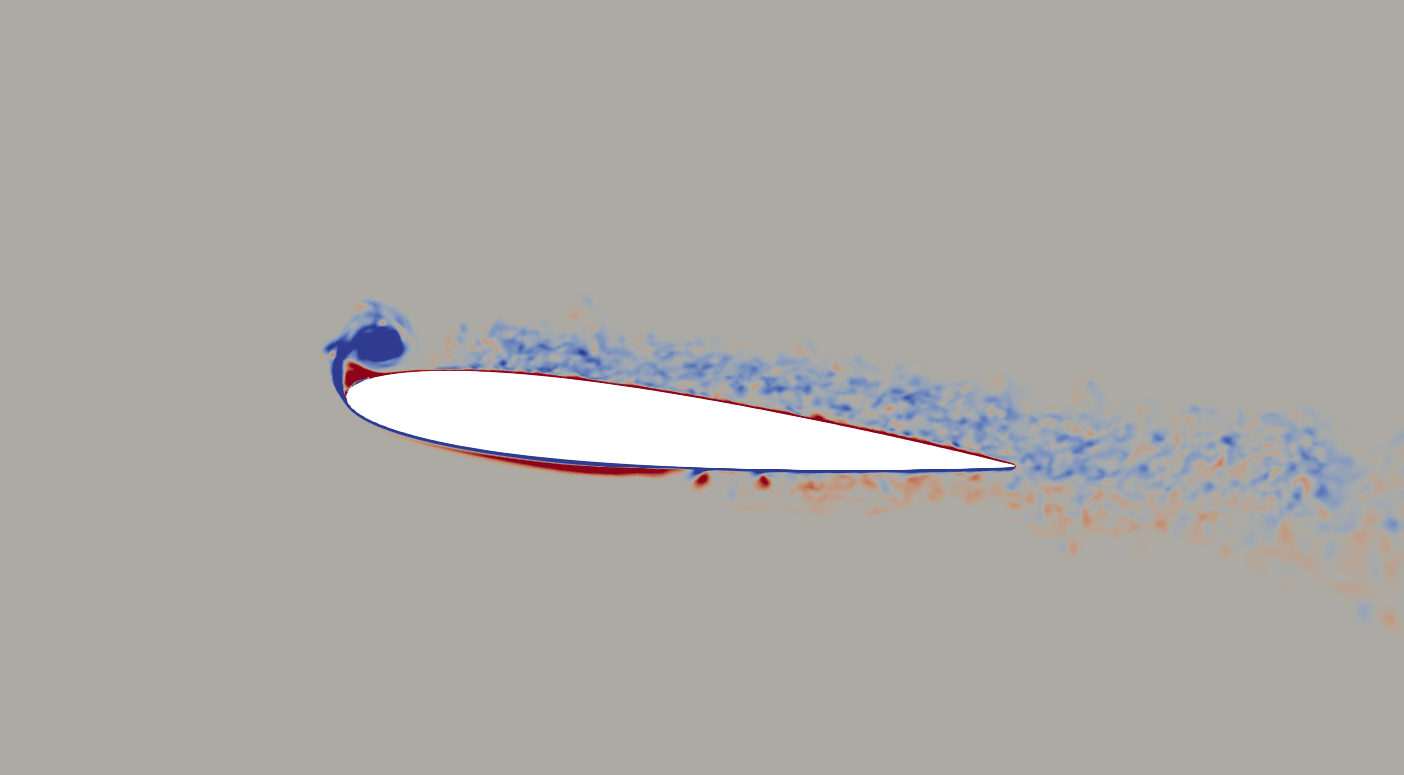
\includegraphics[width=1\textwidth]{figures/zonal_adapt_results/vorticity_plots_Re200k/Mza2_50/phase_240.png}
		\caption{Mza2\_nz50 mesh, $\psi$ = $240^\circ$}
		\label{fig:Mza2_50_Re200k_sp_psi240}
	\end{subfigure}	
	\caption{Spanwise vorticity comparison at $\psi$ = $240^\circ$ for different meshes}
	\label{fig:vorticity_Re200k_sp_240}
\end{figure}

%%=====================================
%% Phase = 255
%%=====================================

%\begin{figure}[H]
%	\centering
%	\begin{center}
%		\begin{subfigure}[b]{0.475\textwidth}
%			\centering
%			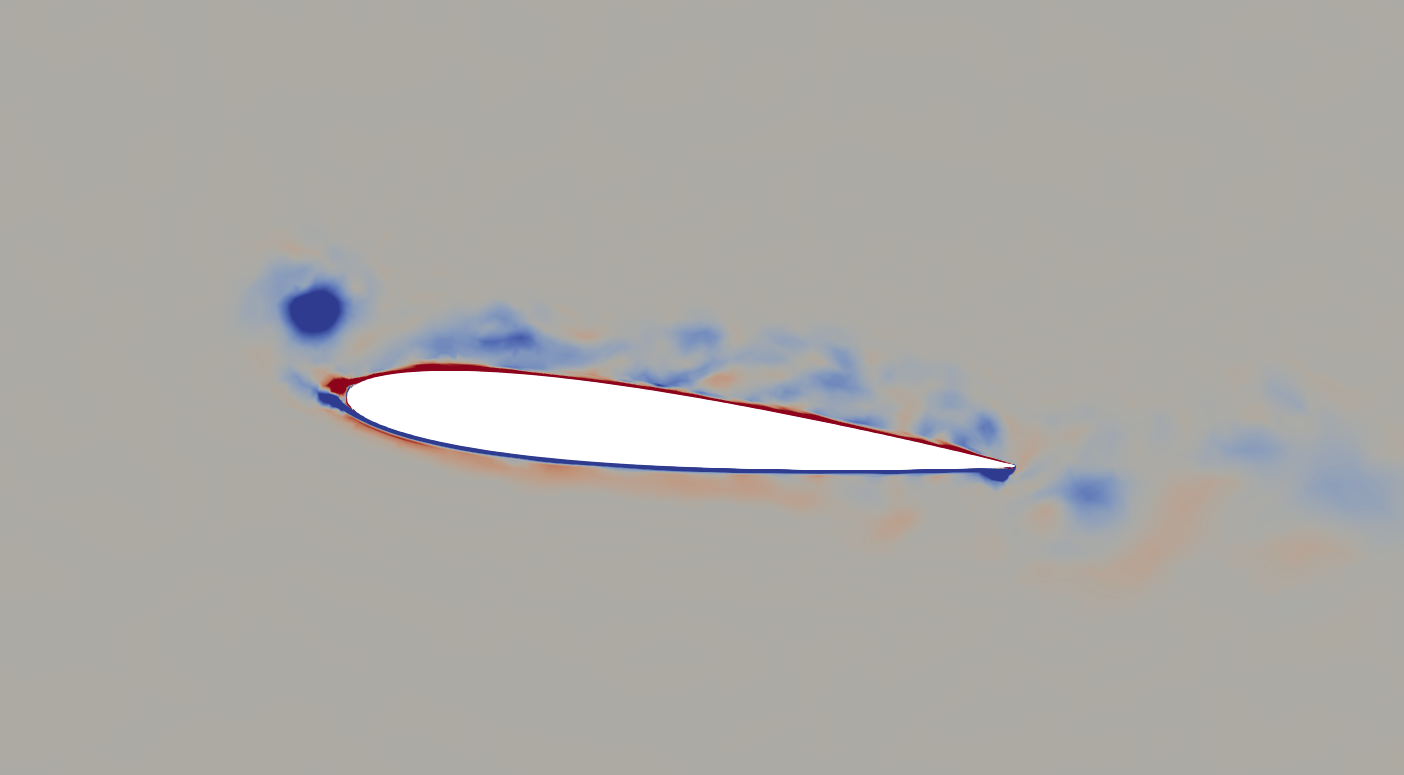
\includegraphics[width=1\textwidth]{figures/zonal_adapt_results/vorticity_plots_Re200k/M0/phase_255.png}
%			\caption{M0 mesh, $\psi$ = $255^\circ$}
%			\label{fig:M0_Re200k_sp_psi255}
%		\end{subfigure}
%	\end{center}
%	\begin{subfigure}[b]{0.475\textwidth}
%		\centering
%		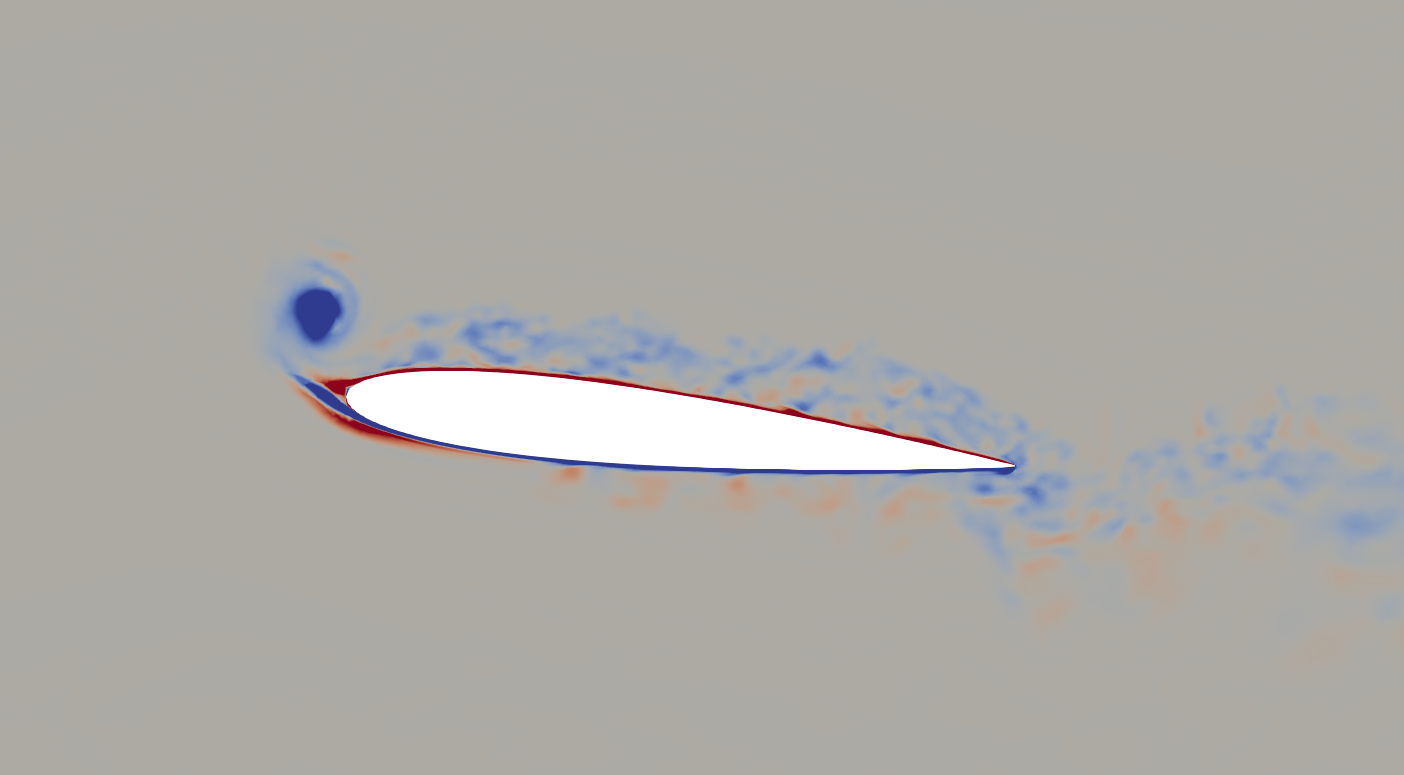
\includegraphics[width=1\textwidth]{figures/zonal_adapt_results/vorticity_plots_Re200k/Mza1_50/phase_255.png}
%		\caption{Mza1\_25 mesh, $\psi$ = $255^\circ$}
%		\label{fig:Mza1_50_Re200k_sp_psi255}
%	\end{subfigure}
%	\begin{subfigure}[b]{0.475\textwidth}
%		\centering
%		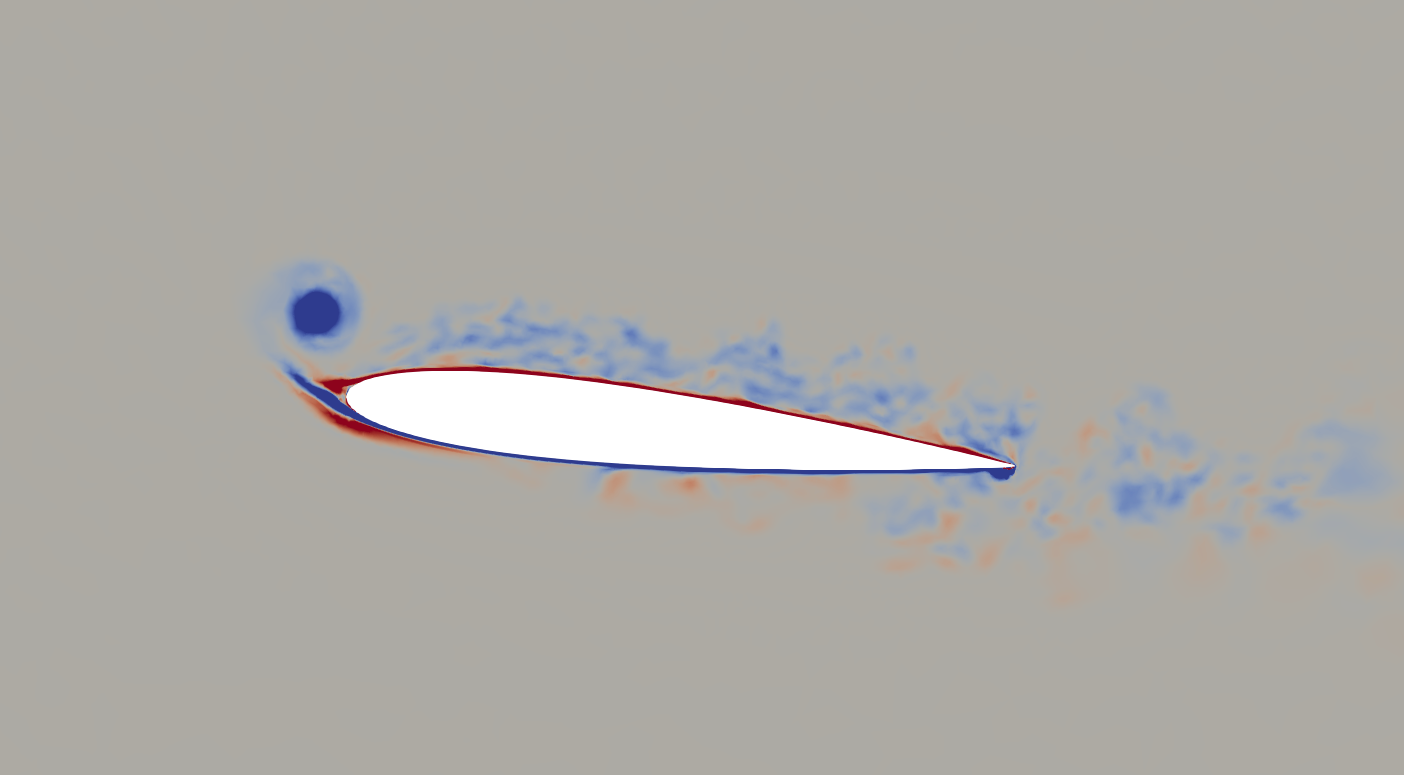
\includegraphics[width=1\textwidth]{figures/zonal_adapt_results/vorticity_plots_Re200k/Mza1_100/phase_255.png}
%		\caption{Mza1\_100 mesh, $\psi$ = $255^\circ$}
%		\label{fig:Mza1_100_Re200k_sp_psi255}
%	\end{subfigure}
%	%	\begin{subfigure}[b]{0.475\textwidth}
%		%		\centering
%		%		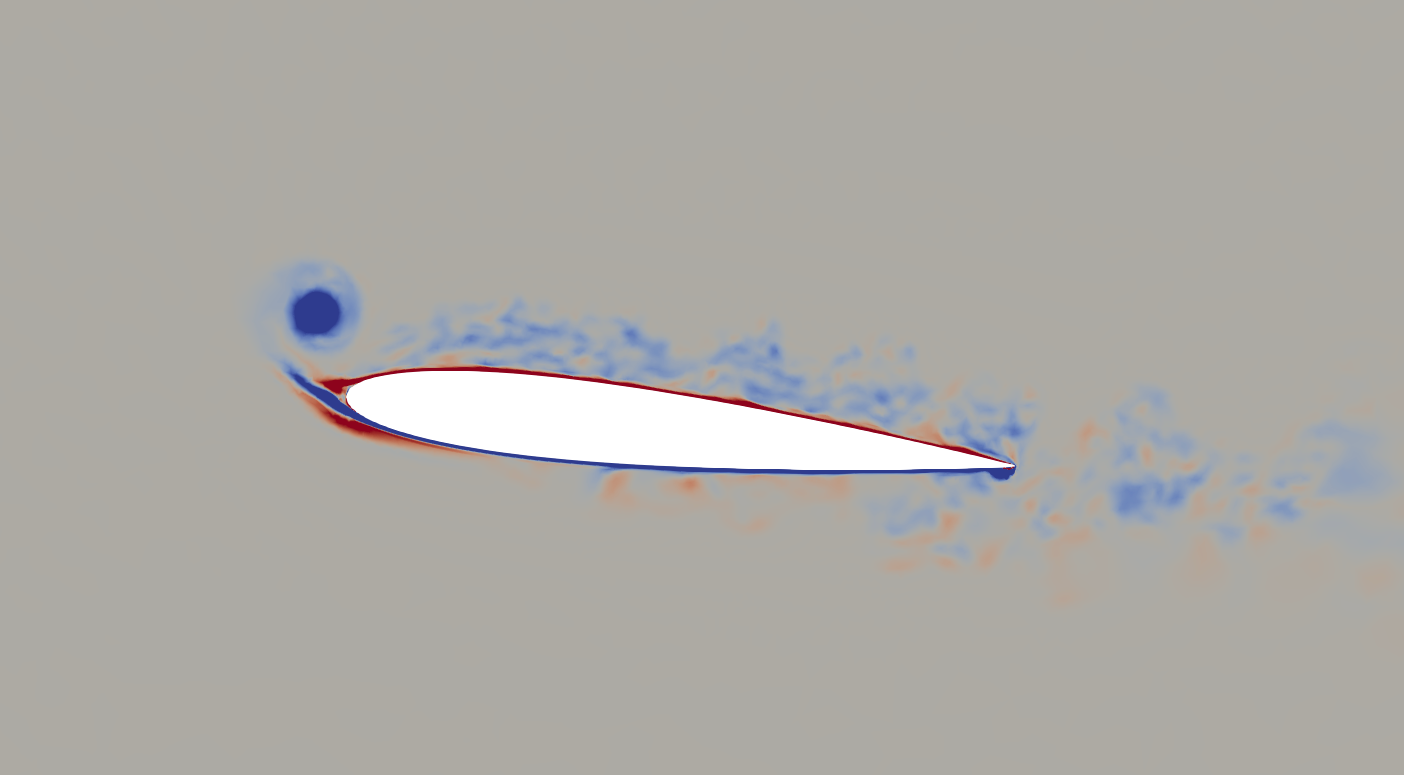
\includegraphics[width=1\textwidth]{figures/zonal_adapt_results/vorticity_plots_Re200k/Mza1_100/phase_255.png}
%		%		\caption{Mza1\_100 mesh, $\psi$ = $255^\circ$}
%		%		\label{fig:Mza1_100_Re200k_sp_psi255}
%		%	\end{subfigure}
%	%	\begin{subfigure}[b]{0.475\textwidth}
%		%	\centering
%		%	\includegraphics[width=1\textwidth]{figures/zonal_adapt_results/vorticity_plots_Re200k/Mza2_25/phase_255.png}
%		%	\caption{Mza2\_25 mesh, $\psi$ = $255^\circ$}
%		%	\label{fig:Mza2_25_Re200k_sp_psi255}
%		%	\end{subfigure}
%	\begin{subfigure}[b]{0.475\textwidth}
%		\centering
%		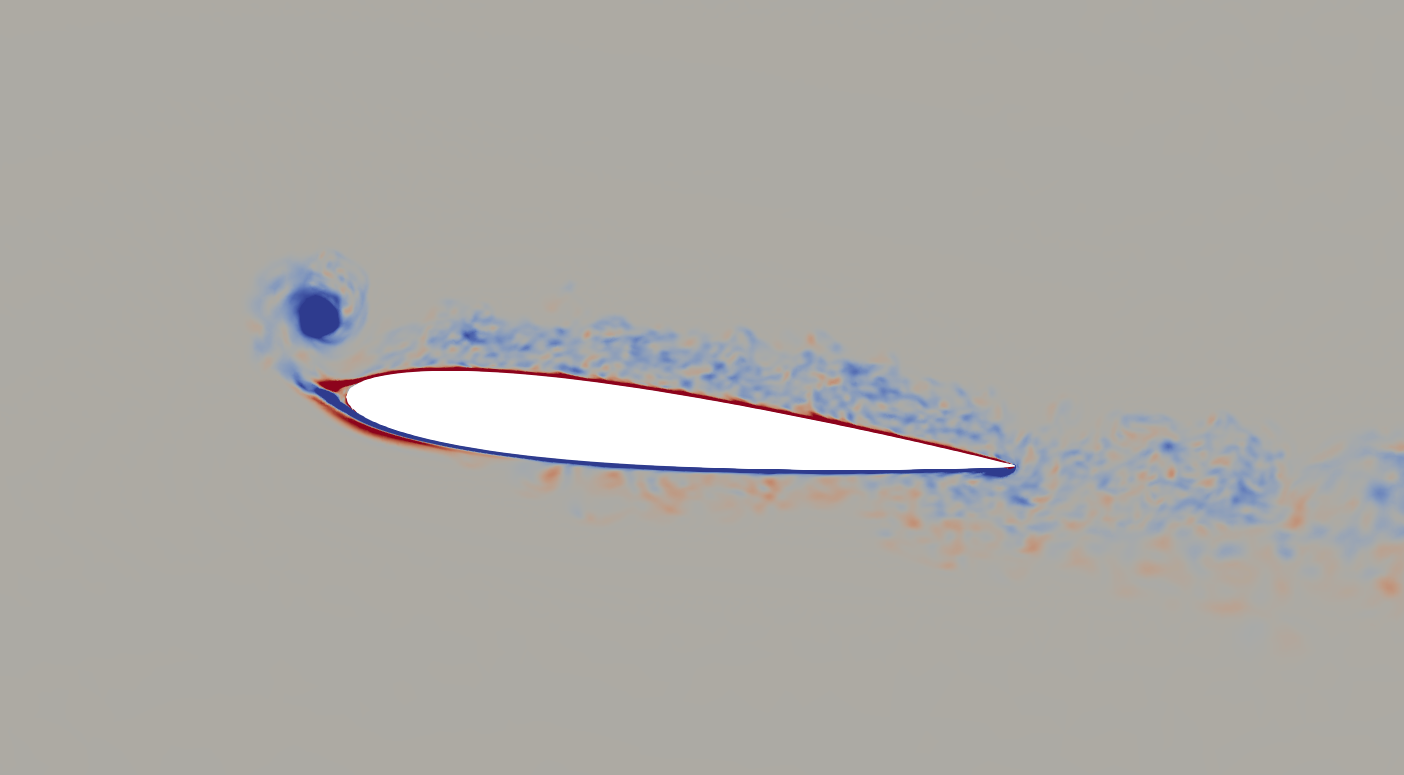
\includegraphics[width=1\textwidth]{figures/zonal_adapt_results/vorticity_plots_Re200k/Mza2_50/phase_255.png}
%		\caption{Mza2\_50 mesh, $\psi$ = $255^\circ$}
%		\label{fig:Mza2_50_Re200k_sp_psi255}
%	\end{subfigure}	
%	%	\begin{subfigure}[b]{0.475\textwidth}
%		%		\centering
%		%		\includegraphics[width=1\textwidth]{figures/zonal_adapt_results/vorticity_plots_Re200k/Mza2_100/phase_255.png}
%		%		\caption{Mza2\_100 mesh, $\psi$ = $255^\circ$}
%		%		\label{fig:Mza2_100_Re200k_sp_psi255}
%		%	\end{subfigure}
%	%	\begin{subfigure}[b]{0.475\textwidth}
%		%	\centering
%		%	\includegraphics[width=1\textwidth]{figures/zonal_adapt_results/vorticity_plots_Re200k/Mza3_50/phase_255.png}
%		%	\caption{Mza3\_50 mesh, $\psi$ = $255^\circ$}
%		%	\label{fig:Mza3_100_Re200k_sp_psi255}
%		%	\end{subfigure}
%	%	\begin{subfigure}[b]{0.475\textwidth}
%		%		\centering
%		%		\includegraphics[width=1\textwidth]{figures/zonal_adapt_results/vorticity_plots_Re200k/Mza3_100/phase_255.png}
%		%		\caption{Mza3\_100 mesh, $\psi$ = $255^\circ$}
%		%		\label{fig:Mza3_100_Re200k_sp_psi255}
%		%	\end{subfigure}
%	\caption{Spanwise vorticity comparison at $\psi$ = $255^\circ$ for different meshes}
%	\label{fig:vorticity_Re200k_sp_255}
%\end{figure}




%%=====================================
%% Phase = 270
%%=====================================

\begin{figure}[H]
	\centering
	\begin{center}
		\begin{subfigure}[b]{0.6\textwidth}
			\centering
			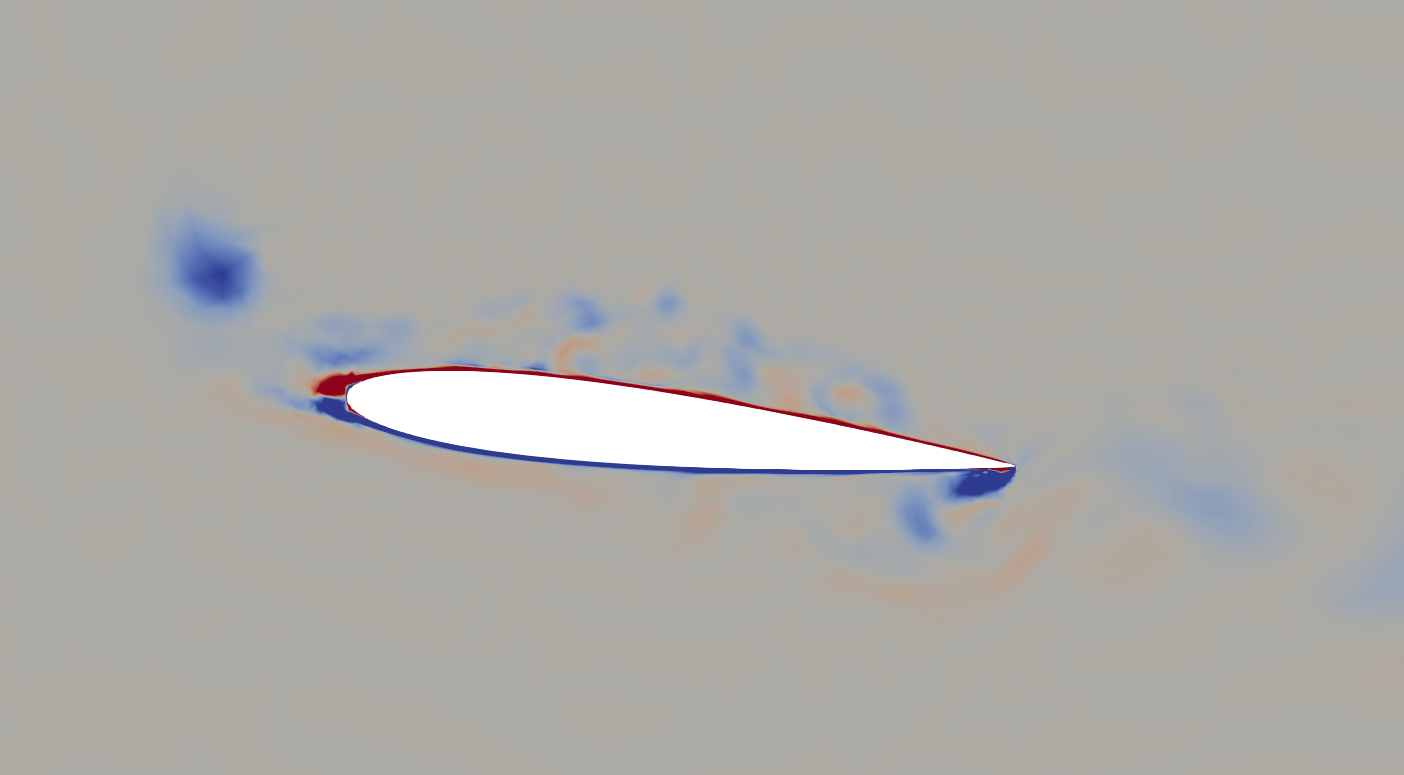
\includegraphics[width=1\textwidth]{figures/zonal_adapt_results/vorticity_plots_Re200k/M0/phase_270.png}
			\caption{M0\_nz50 mesh, $\psi$ = $270^\circ$}
			\label{fig:M0_Re200k_sp_psi270}
		\end{subfigure}
	\end{center}
	\begin{subfigure}[b]{0.6\textwidth}
		\centering
		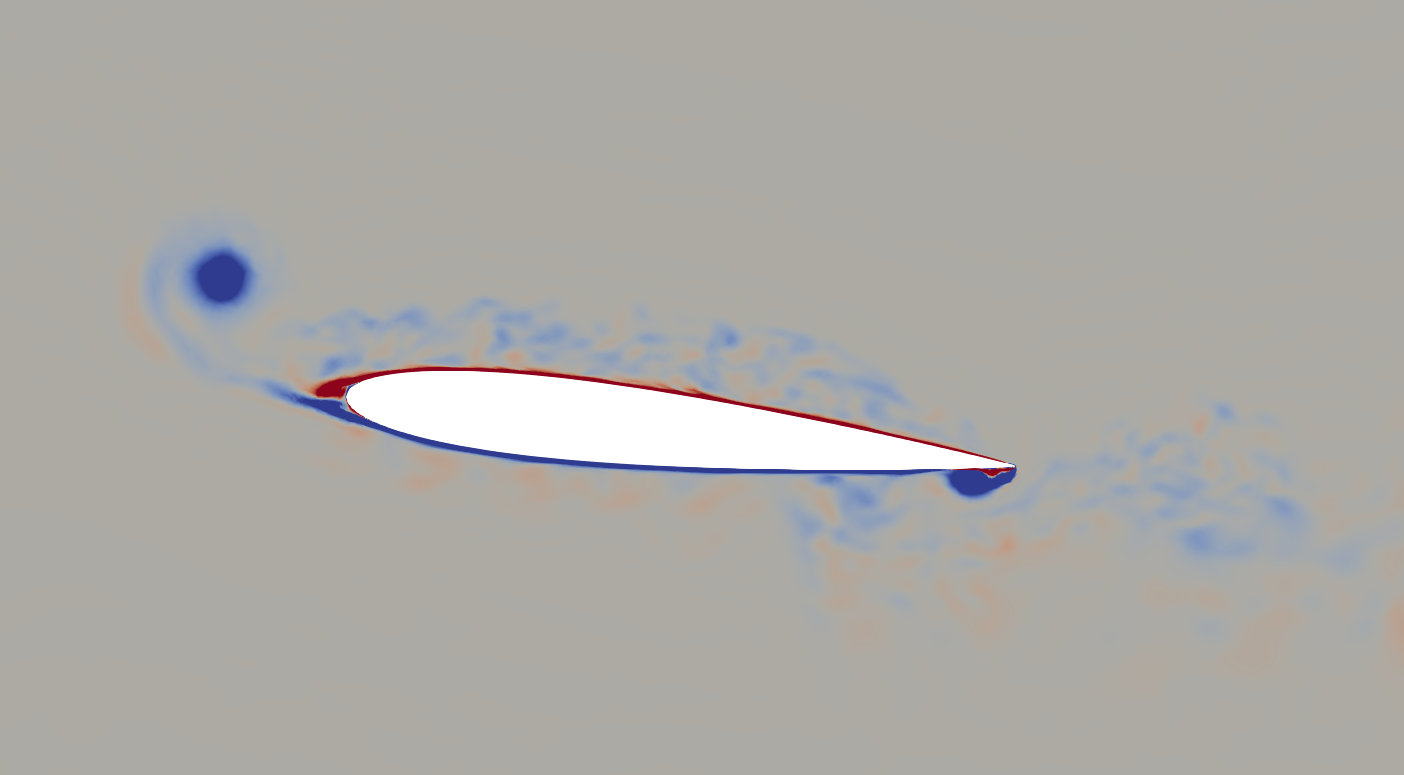
\includegraphics[width=1\textwidth]{figures/zonal_adapt_results/vorticity_plots_Re200k/Mza1_50/phase_270.png}
		\caption{Mza1\_nz50 mesh, $\psi$ = $270^\circ$}
		\label{fig:Mza1_50_Re200k_sp_psi270}
	\end{subfigure}
	%	\begin{subfigure}[b]{0.475\textwidth}
		%		\centering
		%		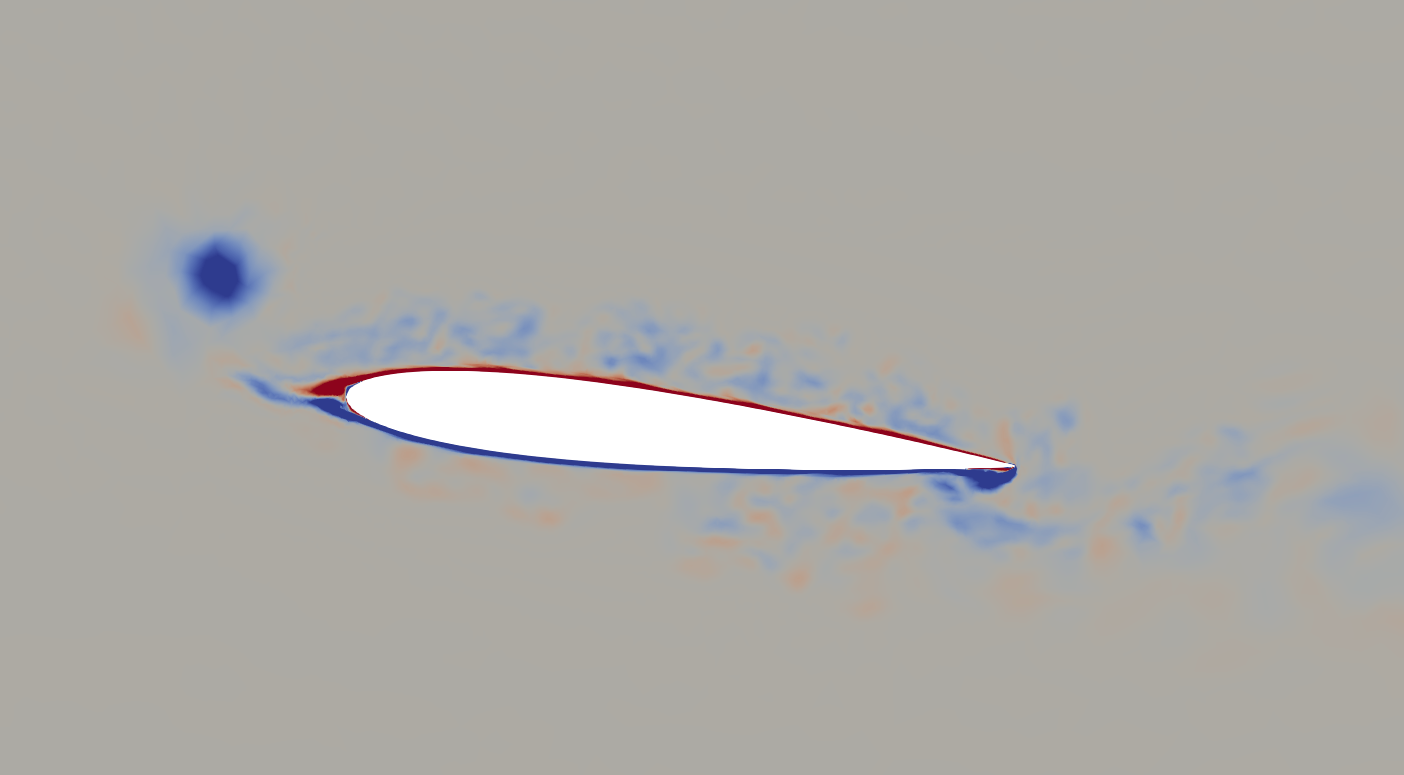
\includegraphics[width=1\textwidth]{figures/zonal_adapt_results/vorticity_plots_Re200k/Mza1_100/phase_270.png}
		%		\caption{Mza1\_100 mesh, $\psi$ = $270^\circ$}
		%		\label{fig:Mza1_100_Re200k_sp_psi270}
		%	\end{subfigure}
	\begin{subfigure}[b]{0.6\textwidth}
		\centering
		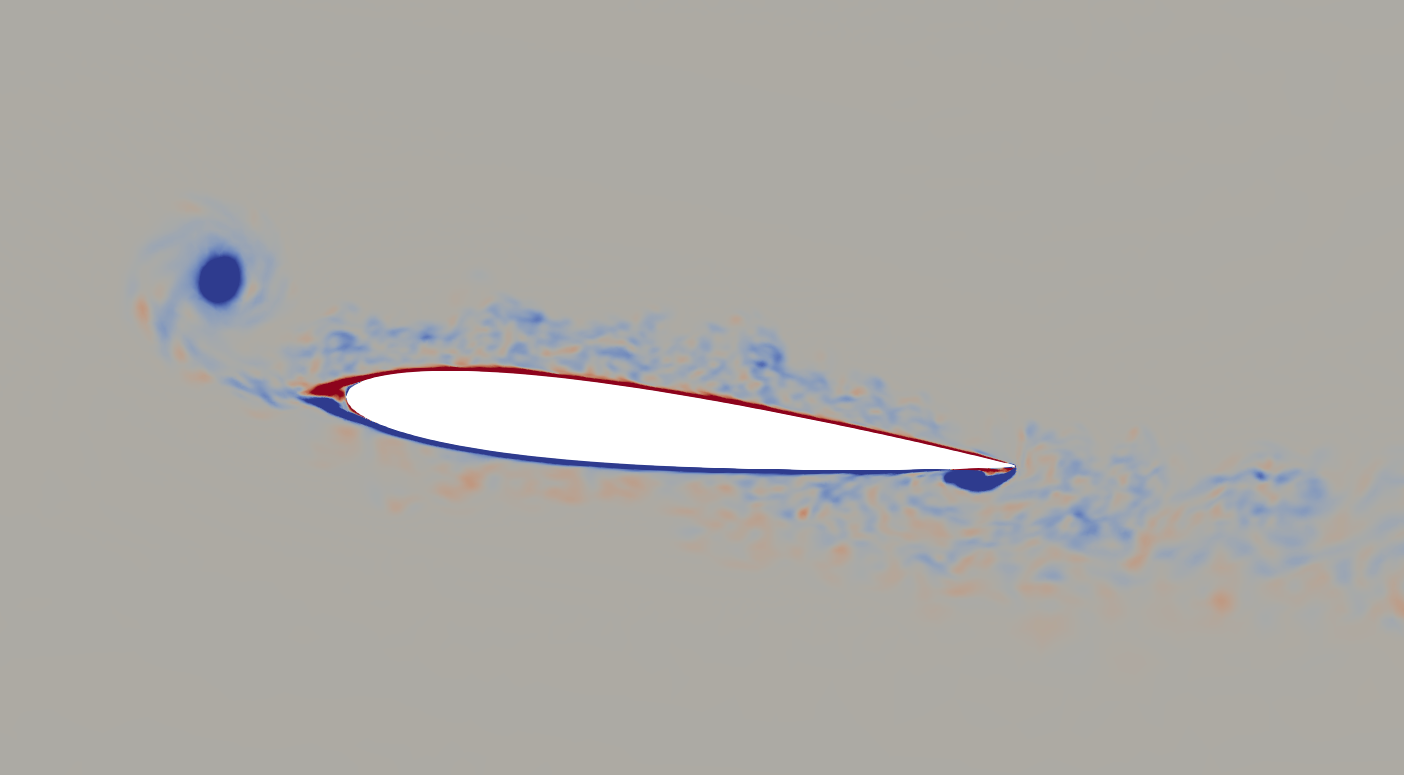
\includegraphics[width=1\textwidth]{figures/zonal_adapt_results/vorticity_plots_Re200k/Mza2_50/phase_270.png}
		\caption{Mza2\_nz50 mesh, $\psi$ = $270^\circ$}
		\label{fig:Mza2_50_Re200k_sp_psi270}
	\end{subfigure}	
	\caption{Spanwise vorticity comparison at $\psi$ = $270^\circ$ for different meshes}
	\label{fig:vorticity_Re200k_sp_270}
\end{figure}

%%=====================================
%% Phase = 285
%%=====================================

%\begin{figure}[H]
%	\centering
%	\begin{center}
%		\begin{subfigure}[b]{0.475\textwidth}
%			\centering
%			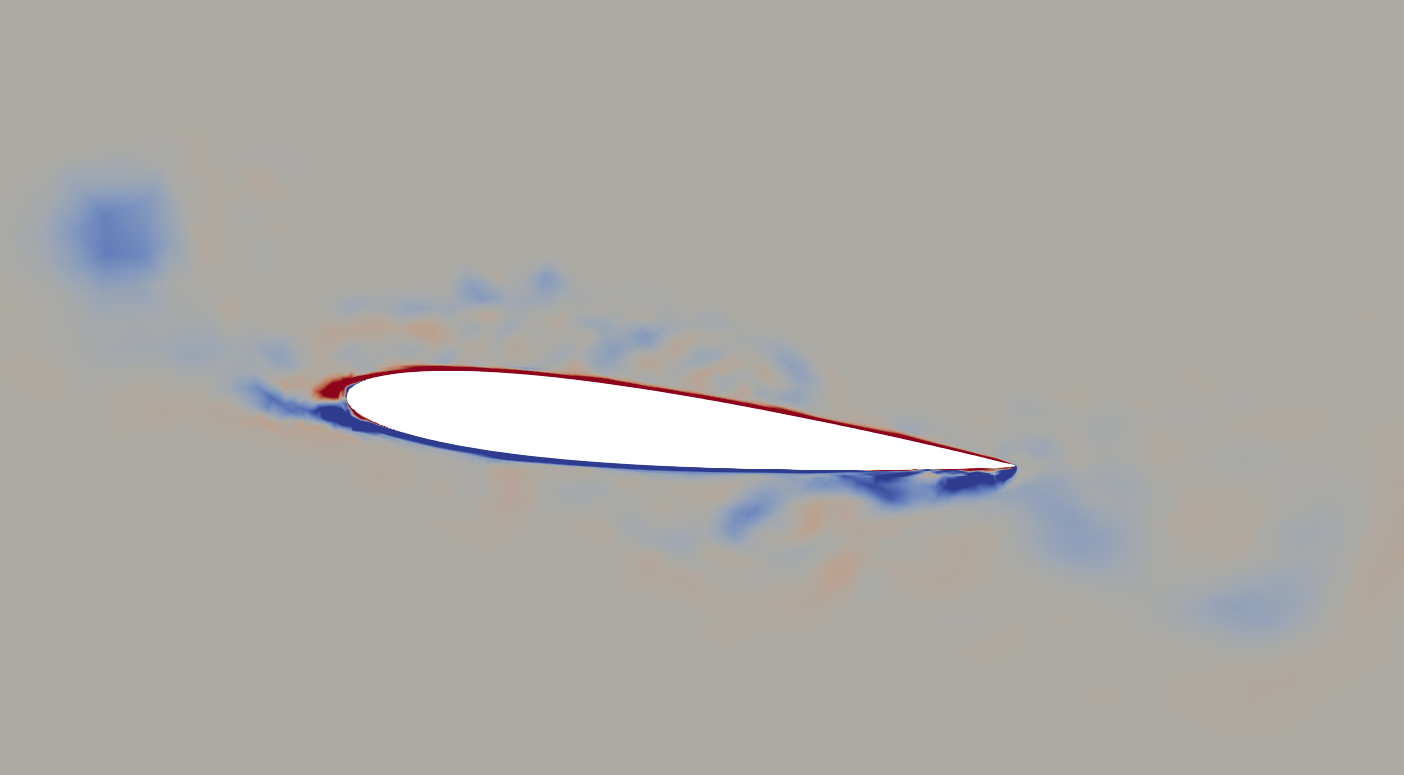
\includegraphics[width=1\textwidth]{figures/zonal_adapt_results/vorticity_plots_Re200k/M0/phase_285.png}
%			\caption{M0 mesh, $\psi$ = $285^\circ$}
%			\label{fig:M0_Re200k_sp_psi285}
%		\end{subfigure}
%	\end{center}
%	\begin{subfigure}[b]{0.475\textwidth}
%		\centering
%		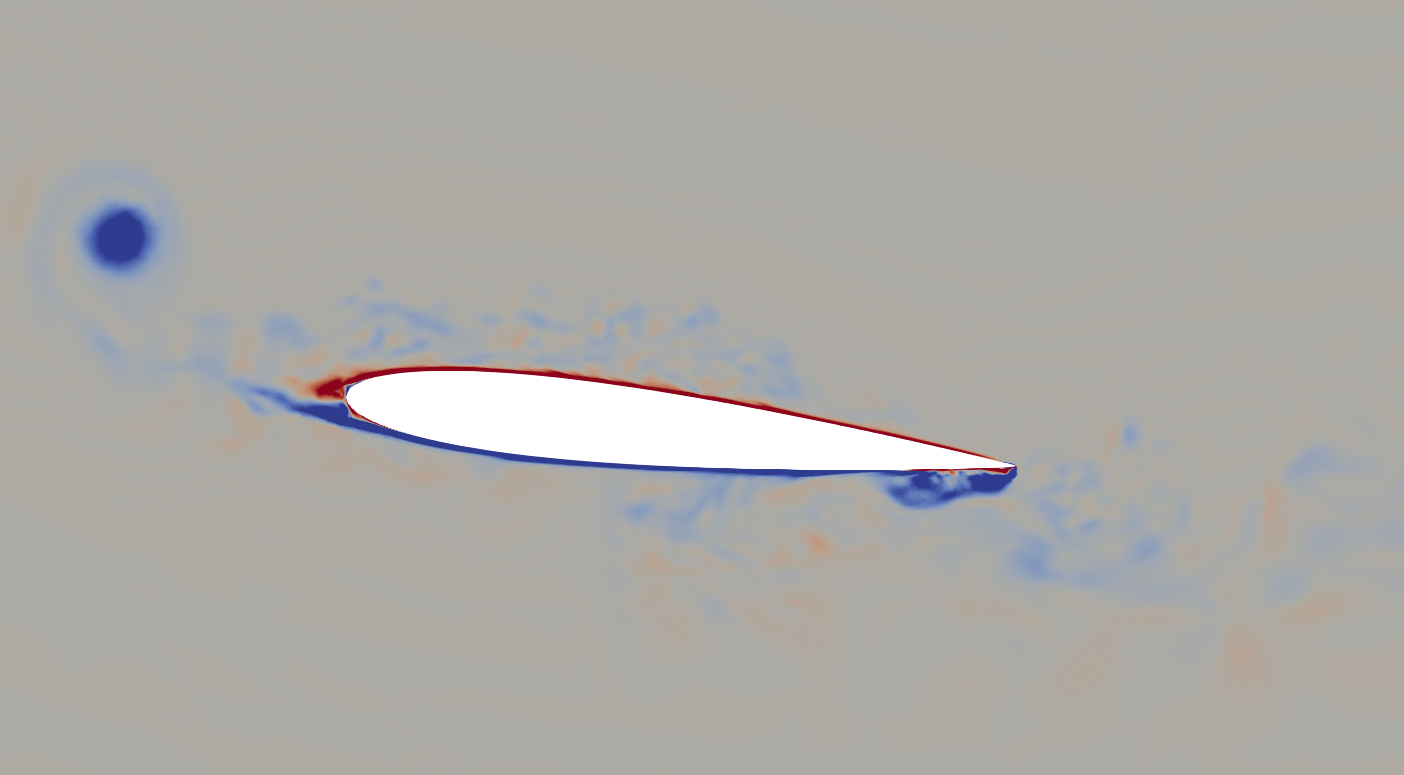
\includegraphics[width=1\textwidth]{figures/zonal_adapt_results/vorticity_plots_Re200k/Mza1_50/phase_285.png}
%		\caption{Mza1\_25 mesh, $\psi$ = $285^\circ$}
%		\label{fig:Mza1_50_Re200k_sp_psi285}
%	\end{subfigure}
%	\begin{subfigure}[b]{0.475\textwidth}
%		\centering
%		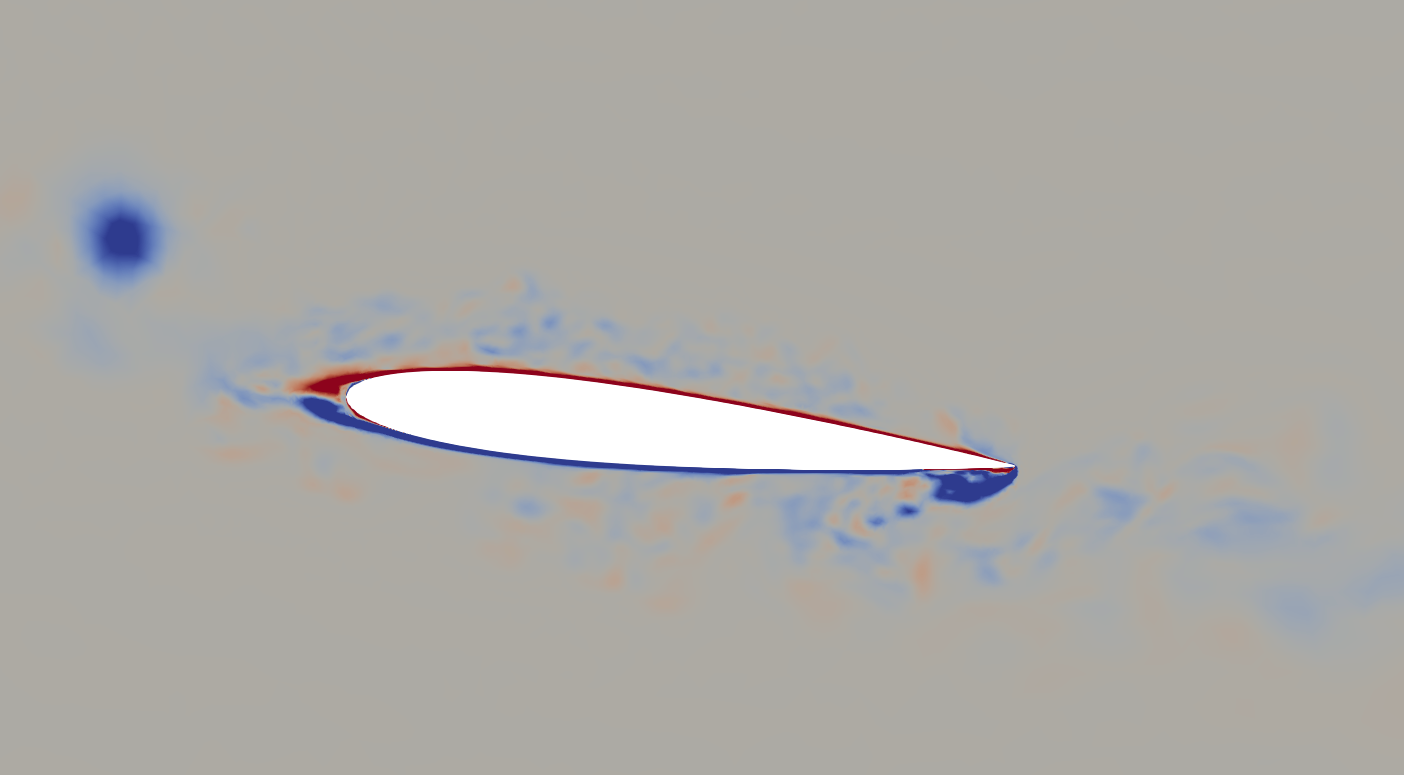
\includegraphics[width=1\textwidth]{figures/zonal_adapt_results/vorticity_plots_Re200k/Mza1_100/phase_285.png}
%		\caption{Mza1\_100 mesh, $\psi$ = $285^\circ$}
%		\label{fig:Mza1_100_Re200k_sp_psi285}
%	\end{subfigure}
%	%	\begin{subfigure}[b]{0.475\textwidth}
%		%		\centering
%		%		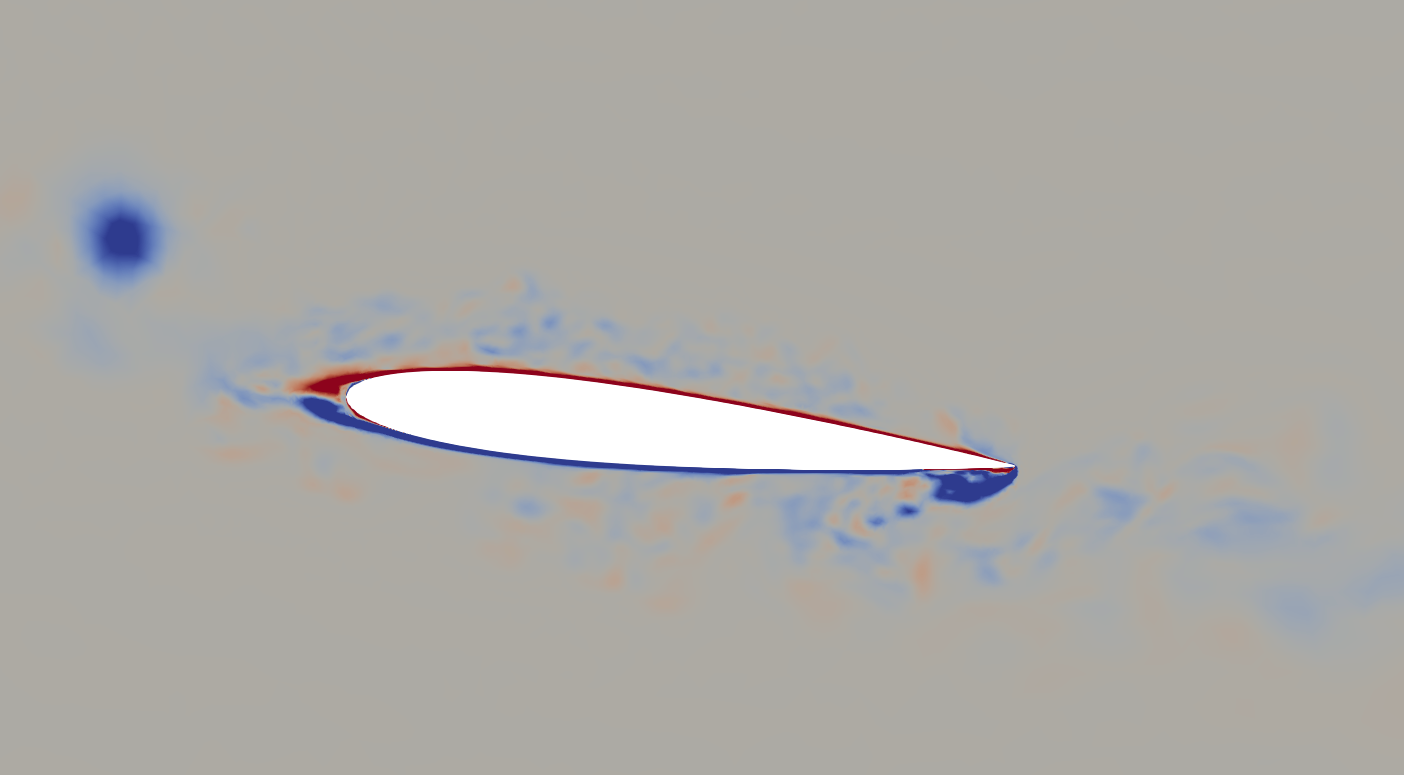
\includegraphics[width=1\textwidth]{figures/zonal_adapt_results/vorticity_plots_Re200k/Mza1_100/phase_285.png}
%		%		\caption{Mza1\_100 mesh, $\psi$ = $285^\circ$}
%		%		\label{fig:Mza1_100_Re200k_sp_psi285}
%		%	\end{subfigure}
%	%	\begin{subfigure}[b]{0.475\textwidth}
%		%	\centering
%		%	\includegraphics[width=1\textwidth]{figures/zonal_adapt_results/vorticity_plots_Re200k/Mza2_25/phase_285.png}
%		%	\caption{Mza2\_25 mesh, $\psi$ = $285^\circ$}
%		%	\label{fig:Mza2_25_Re200k_sp_psi285}
%		%	\end{subfigure}
%	\begin{subfigure}[b]{0.475\textwidth}
%		\centering
%		\includegraphics[width=1\textwidth]{figures/zonal_adapt_results/vorticity_plots_Re200k/Mza2_50/phase_285.png}
%		\caption{Mza2\_50 mesh, $\psi$ = $285^\circ$}
%		\label{fig:Mza2_50_Re200k_sp_psi285}
%	\end{subfigure}	
%	%	\begin{subfigure}[b]{0.475\textwidth}
%		%		\centering
%		%		\includegraphics[width=1\textwidth]{figures/zonal_adapt_results/vorticity_plots_Re200k/Mza2_100/phase_285.png}
%		%		\caption{Mza2\_100 mesh, $\psi$ = $285^\circ$}
%		%		\label{fig:Mza2_100_Re200k_sp_psi285}
%		%	\end{subfigure}
%	%	\begin{subfigure}[b]{0.475\textwidth}
%		%	\centering
%		%	\includegraphics[width=1\textwidth]{figures/zonal_adapt_results/vorticity_plots_Re200k/Mza3_50/phase_285.png}
%		%	\caption{Mza3\_50 mesh, $\psi$ = $285^\circ$}
%		%	\label{fig:Mza3_100_Re200k_sp_psi285}
%		%	\end{subfigure}
%	%	\begin{subfigure}[b]{0.475\textwidth}
%		%		\centering
%		%		\includegraphics[width=1\textwidth]{figures/zonal_adapt_results/vorticity_plots_Re200k/Mza3_100/phase_285.png}
%		%		\caption{Mza3\_100 mesh, $\psi$ = $285^\circ$}
%		%		\label{fig:Mza3_100_Re200k_sp_psi285}
%		%	\end{subfigure}
%	\caption{Spanwise vorticity comparison at $\psi$ = $285^\circ$ for different meshes}
%	\label{fig:vorticity_Re200k_sp_285}
%\end{figure}


%%=====================================
%% Phase = 300
%%=====================================

\begin{figure}[H]
	\centering
	\begin{center}
		\begin{subfigure}[b]{0.6\textwidth}
			\centering
			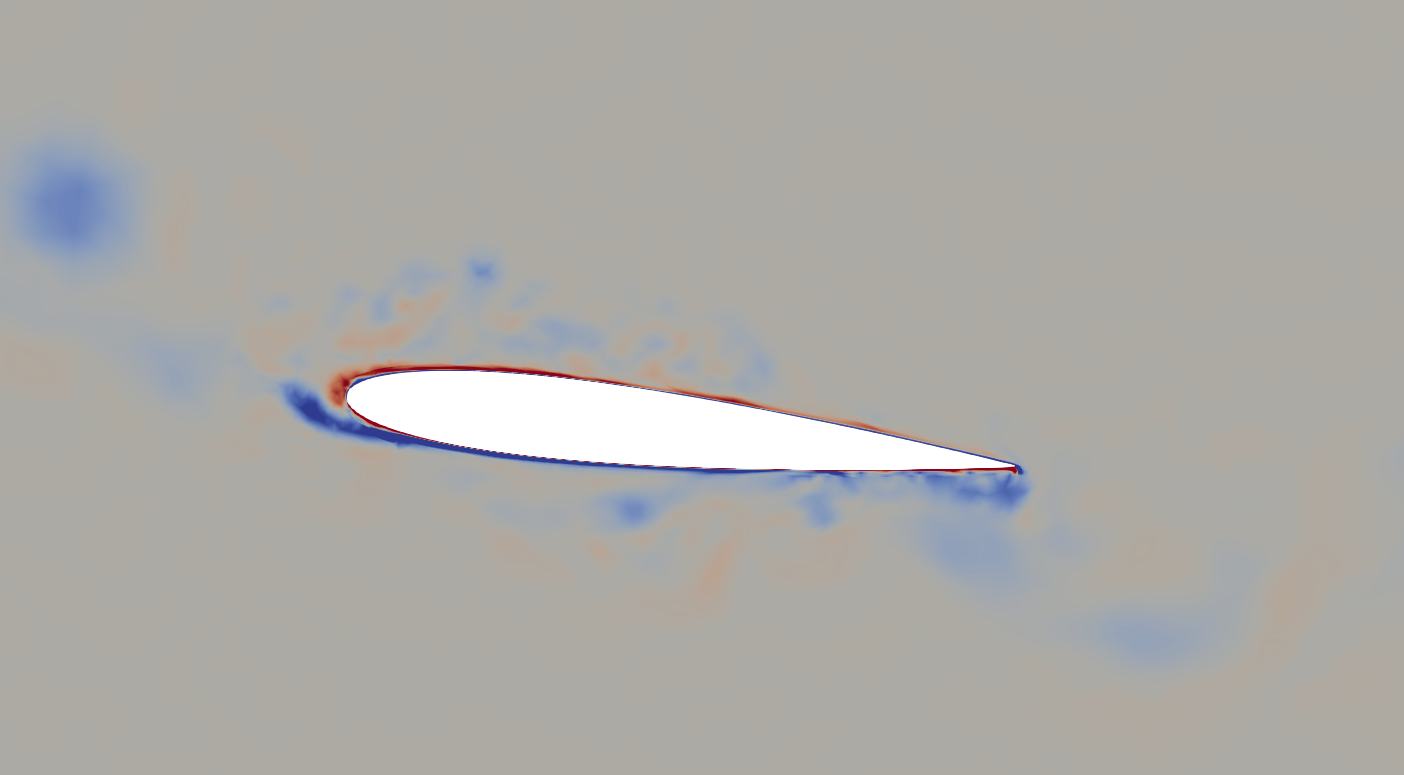
\includegraphics[width=1\textwidth]{figures/zonal_adapt_results/vorticity_plots_Re200k/M0/phase_300.png}
			\caption{M0\_nz50 mesh, $\psi$ = $300^\circ$}
			\label{fig:M0_Re200k_sp_psi300}
		\end{subfigure}
	\end{center}
	\begin{subfigure}[b]{0.6\textwidth}
		\centering
		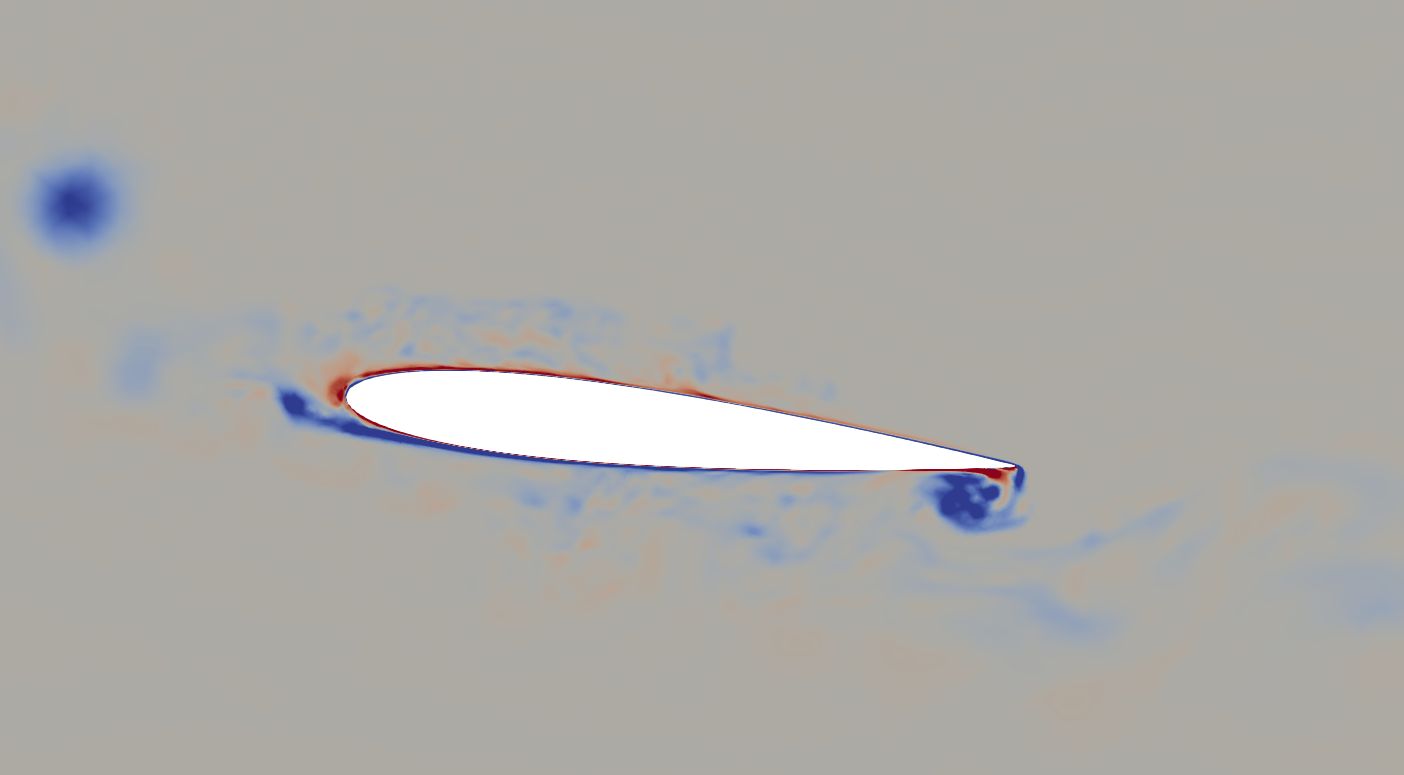
\includegraphics[width=1\textwidth]{figures/zonal_adapt_results/vorticity_plots_Re200k/Mza1_50/phase_300.png}
		\caption{Mza1\_nz50 mesh, $\psi$ = $300^\circ$}
		\label{fig:Mza1_50_Re200k_sp_psi300}
	\end{subfigure}
	%	\begin{subfigure}[b]{0.475\textwidth}
		%		\centering
		%		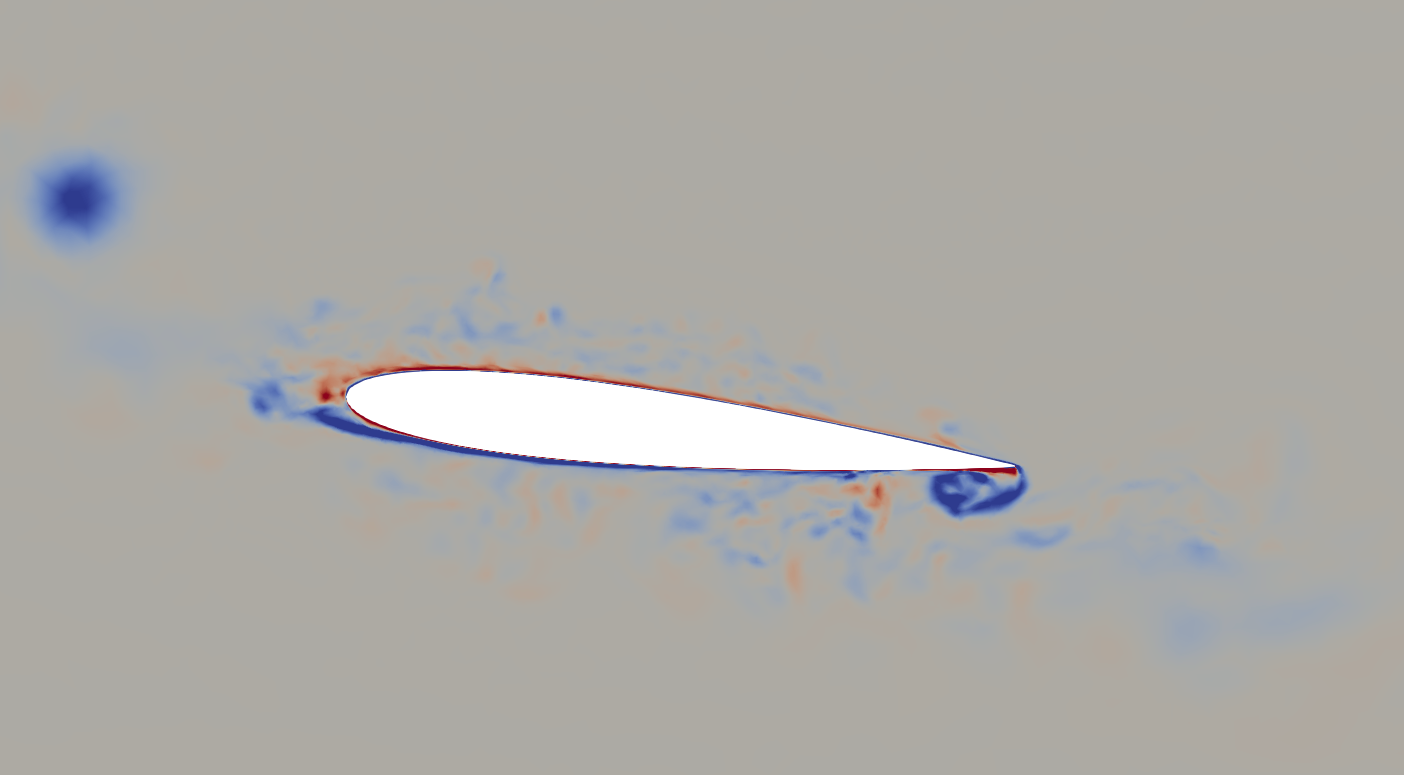
\includegraphics[width=1\textwidth]{figures/zonal_adapt_results/vorticity_plots_Re200k/Mza1_100/phase_300.png}
		%		\caption{Mza1\_100 mesh, $\psi$ = $300^\circ$}
		%		\label{fig:Mza1_100_Re200k_sp_psi300}
		%	\end{subfigure}
	\begin{subfigure}[b]{0.6\textwidth}
		\centering
		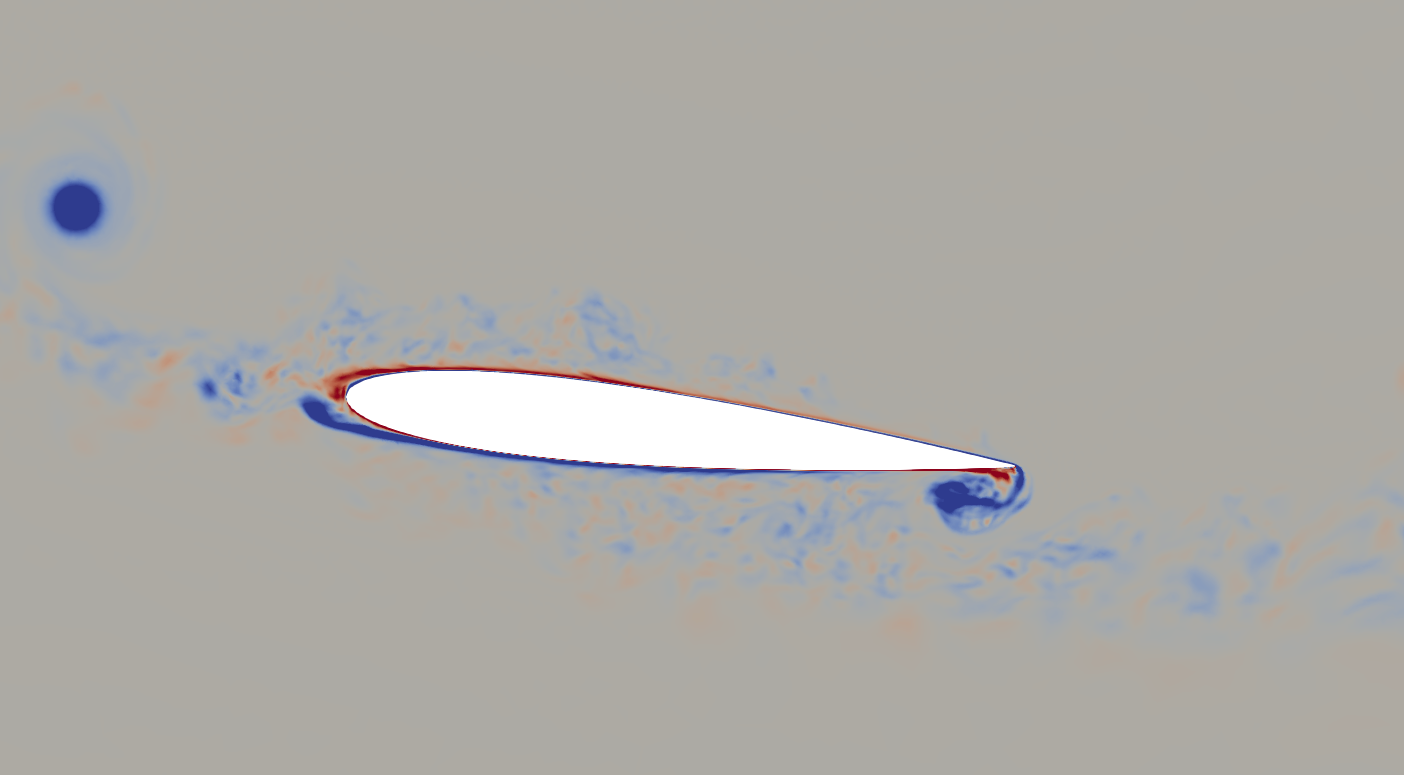
\includegraphics[width=1\textwidth]{figures/zonal_adapt_results/vorticity_plots_Re200k/Mza2_50/phase_300.png}
		\caption{Mza2\_nz50 mesh, $\psi$ = $300^\circ$}
		\label{fig:Mza2_50_Re200k_sp_psi300}
	\end{subfigure}	
	\caption{Spanwise vorticity comparison at $\psi$ = $300^\circ$ for different meshes}
	\label{fig:vorticity_Re200k_sp_300}
\end{figure}
%%=====================================
%% Phase = 315
%%=====================================

%\begin{figure}[H]
%	\centering
%	\begin{center}
%		\begin{subfigure}[b]{0.475\textwidth}
%			\centering
%			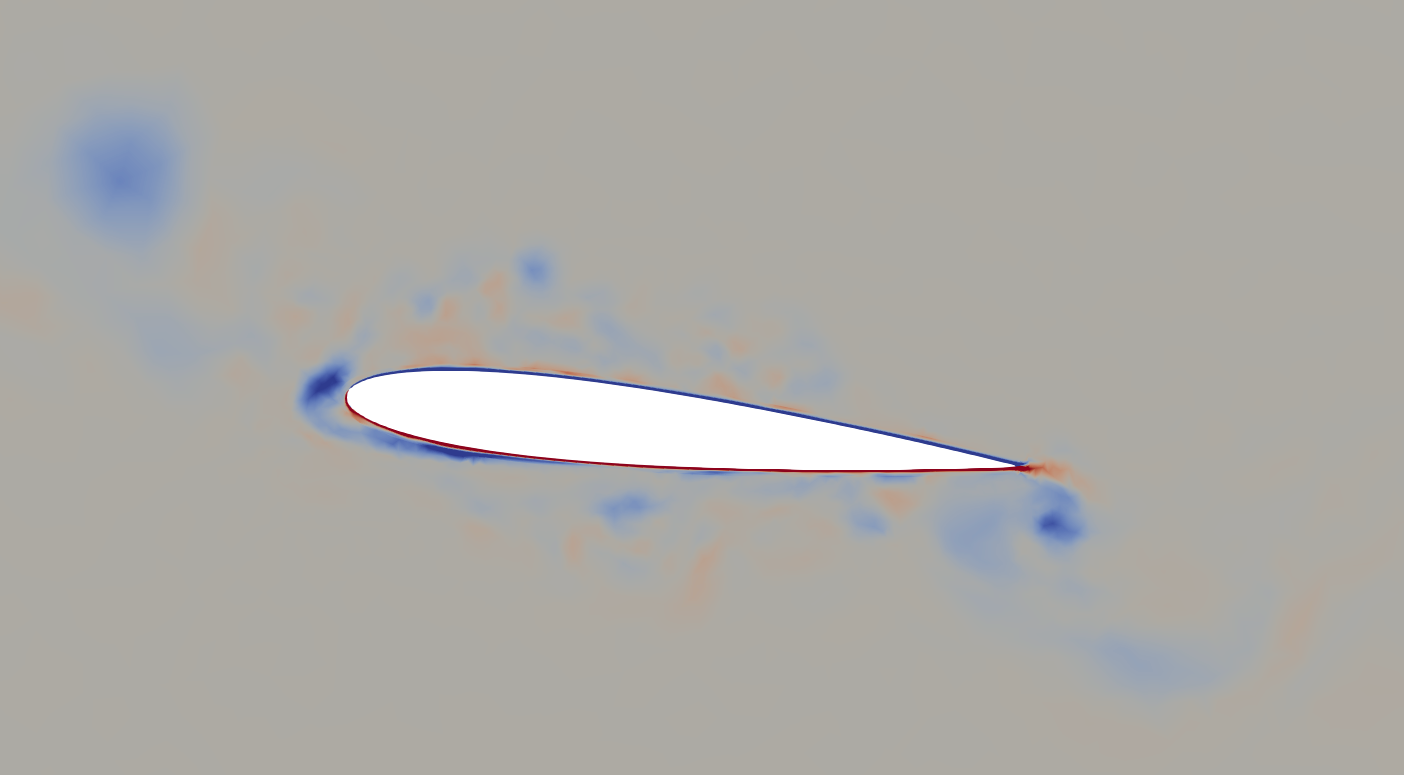
\includegraphics[width=1\textwidth]{figures/zonal_adapt_results/vorticity_plots_Re200k/M0/phase_315.png}
%			\caption{M0 mesh, $\psi$ = $315^\circ$}
%			\label{fig:M0_Re200k_sp_psi315}
%		\end{subfigure}
%	\end{center}
%	\begin{subfigure}[b]{0.475\textwidth}
%		\centering
%		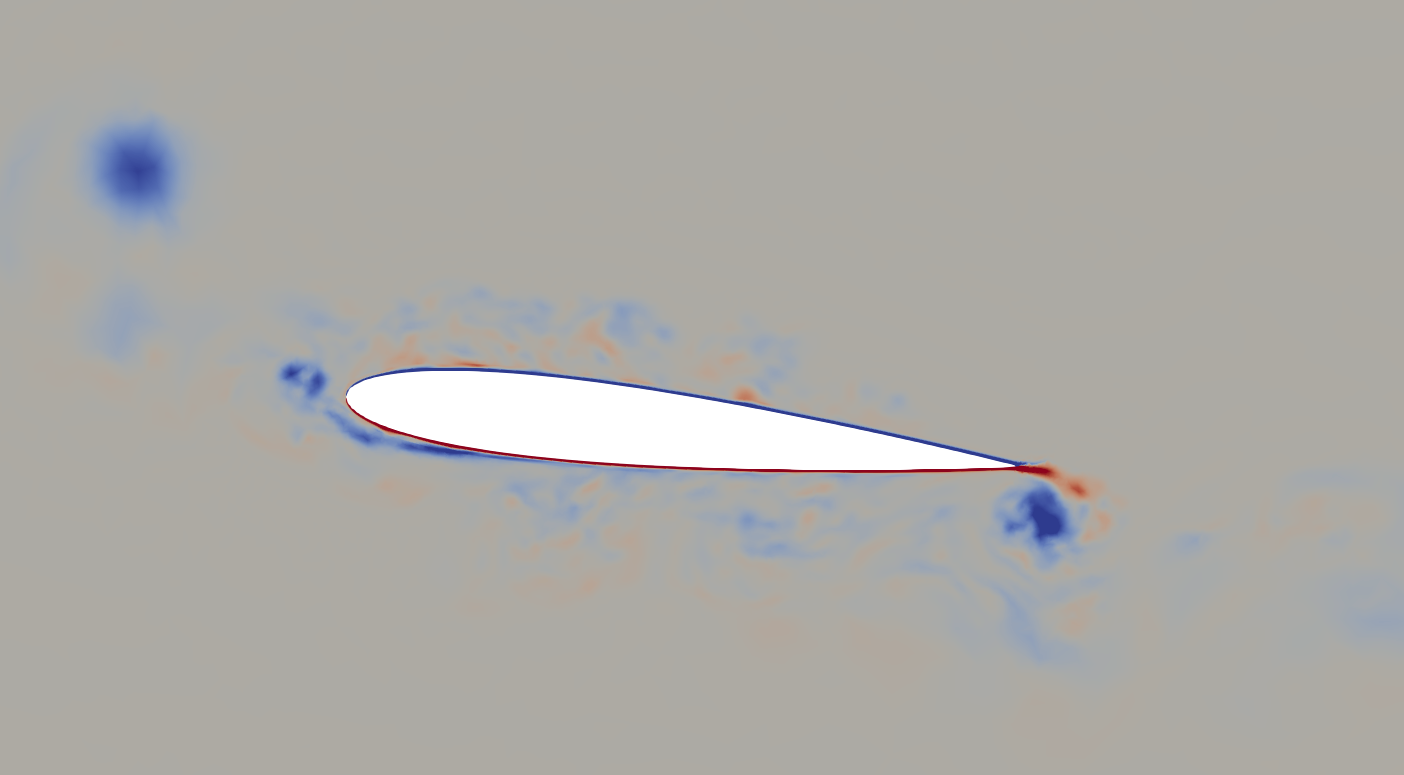
\includegraphics[width=1\textwidth]{figures/zonal_adapt_results/vorticity_plots_Re200k/Mza1_50/phase_315.png}
%		\caption{Mza1\_25 mesh, $\psi$ = $315^\circ$}
%		\label{fig:Mza1_50_Re200k_sp_psi315}
%	\end{subfigure}
%	\begin{subfigure}[b]{0.475\textwidth}
%		\centering
%		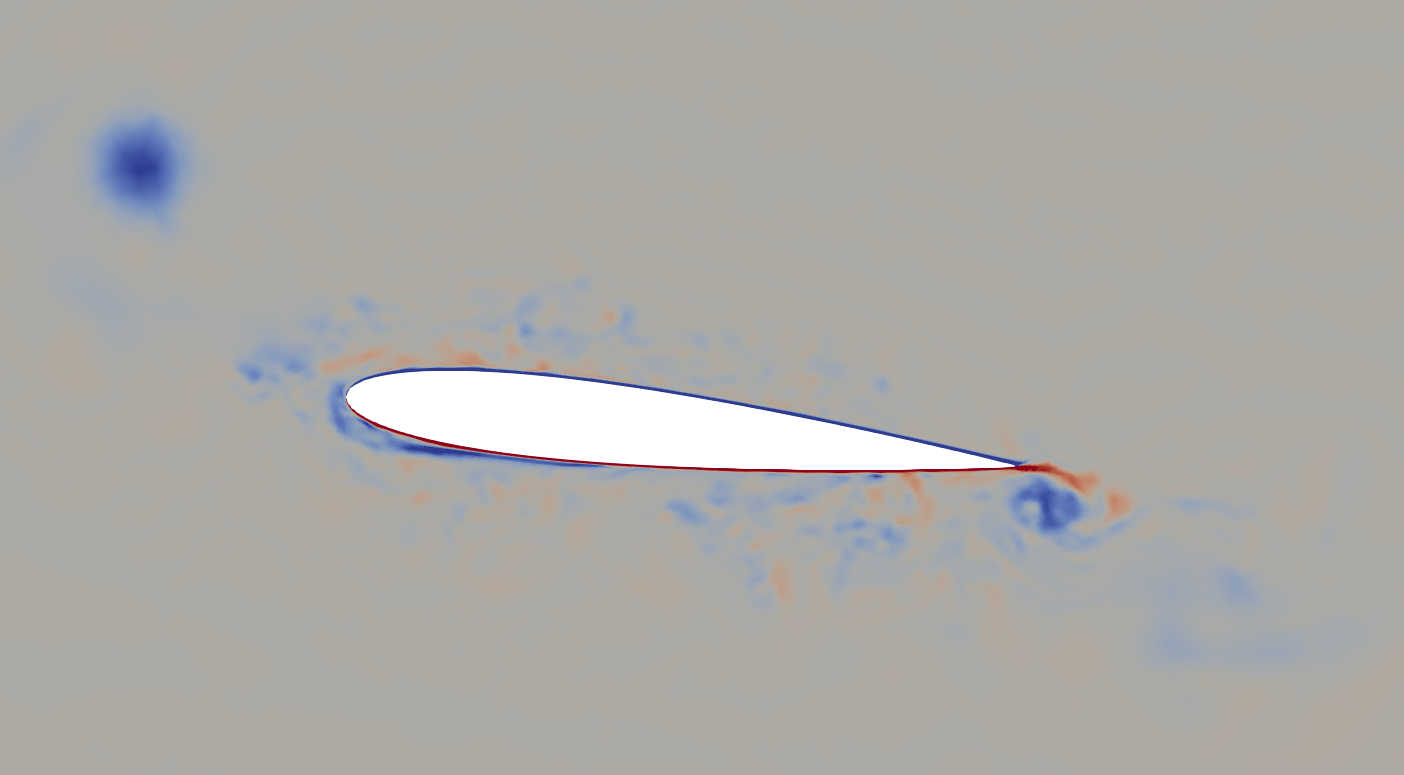
\includegraphics[width=1\textwidth]{figures/zonal_adapt_results/vorticity_plots_Re200k/Mza1_100/phase_315.png}
%		\caption{Mza1\_100 mesh, $\psi$ = $315^\circ$}
%		\label{fig:Mza1_100_Re200k_sp_psi315}
%	\end{subfigure}
%	%	\begin{subfigure}[b]{0.475\textwidth}
%		%		\centering
%		%		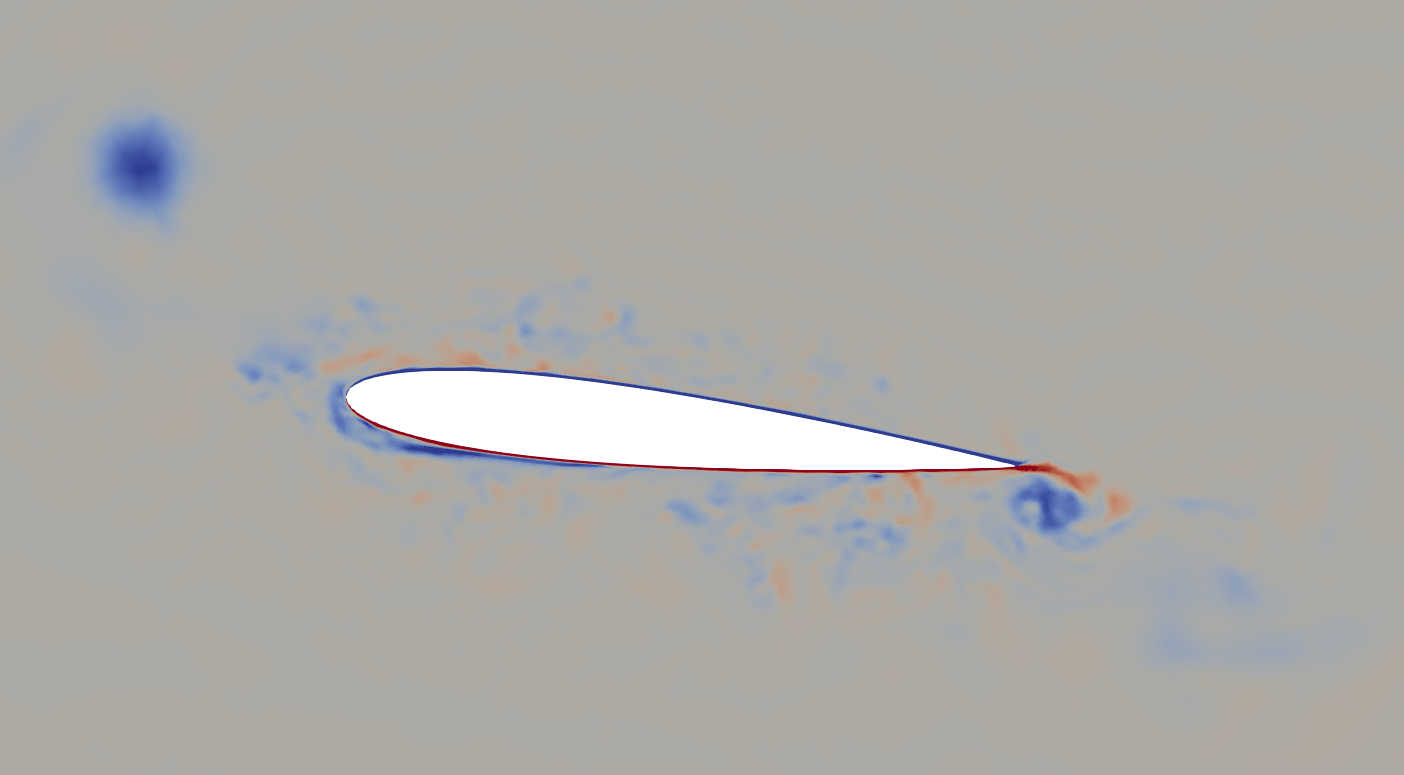
\includegraphics[width=1\textwidth]{figures/zonal_adapt_results/vorticity_plots_Re200k/Mza1_100/phase_315.png}
%		%		\caption{Mza1\_100 mesh, $\psi$ = $315^\circ$}
%		%		\label{fig:Mza1_100_Re200k_sp_psi315}
%		%	\end{subfigure}
%	%	\begin{subfigure}[b]{0.475\textwidth}
%		%	\centering
%		%	\includegraphics[width=1\textwidth]{figures/zonal_adapt_results/vorticity_plots_Re200k/Mza2_25/phase_315.png}
%		%	\caption{Mza2\_25 mesh, $\psi$ = $315^\circ$}
%		%	\label{fig:Mza2_25_Re200k_sp_psi315}
%		%	\end{subfigure}
%	\begin{subfigure}[b]{0.475\textwidth}
%		\centering
%		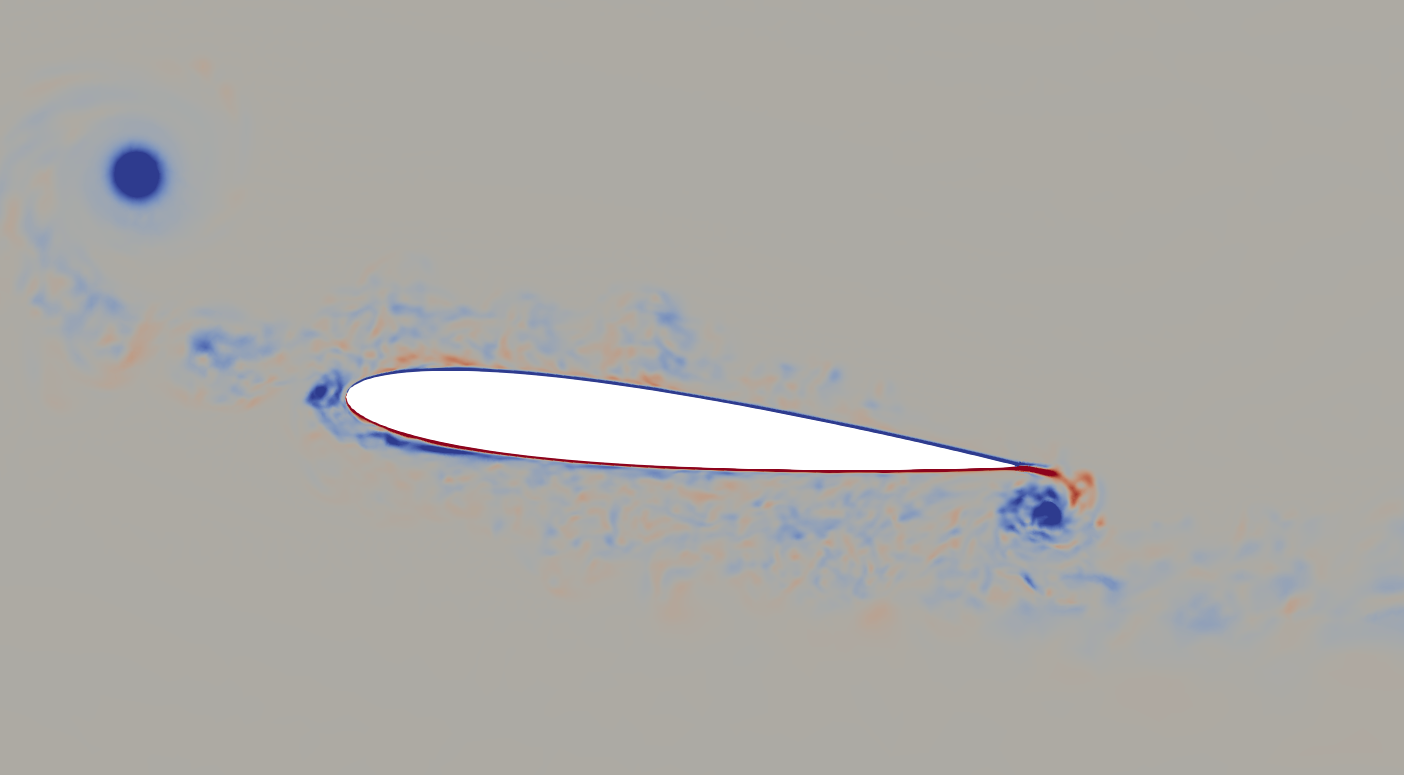
\includegraphics[width=1\textwidth]{figures/zonal_adapt_results/vorticity_plots_Re200k/Mza2_50/phase_315.png}
%		\caption{Mza2\_50 mesh, $\psi$ = $315^\circ$}
%		\label{fig:Mza2_50_Re200k_sp_psi315}
%	\end{subfigure}	
%	%	\begin{subfigure}[b]{0.475\textwidth}
%		%		\centering
%		%		\includegraphics[width=1\textwidth]{figures/zonal_adapt_results/vorticity_plots_Re200k/Mza2_100/phase_315.png}
%		%		\caption{Mza2\_100 mesh, $\psi$ = $315^\circ$}
%		%		\label{fig:Mza2_100_Re200k_sp_psi315}
%		%	\end{subfigure}
%	%	\begin{subfigure}[b]{0.475\textwidth}
%		%	\centering
%		%	\includegraphics[width=1\textwidth]{figures/zonal_adapt_results/vorticity_plots_Re200k/Mza3_50/phase_315.png}
%		%	\caption{Mza3\_50 mesh, $\psi$ = $315^\circ$}
%		%	\label{fig:Mza3_100_Re200k_sp_psi315}
%		%	\end{subfigure}
%	%	\begin{subfigure}[b]{0.475\textwidth}
%		%		\centering
%		%		\includegraphics[width=1\textwidth]{figures/zonal_adapt_results/vorticity_plots_Re200k/Mza3_100/phase_315.png}
%		%		\caption{Mza3\_100 mesh, $\psi$ = $315^\circ$}
%		%		\label{fig:Mza3_100_Re200k_sp_psi315}
%		%	\end{subfigure}
%	\caption{Spanwise vorticity comparison at $\psi$ = $315^\circ$ for different meshes}
%	\label{fig:vorticity_Re200k_sp_315}
=======
In this section, a comparison of instantaneous spanwise vorticity for the different meshes is shown in Figures \ref{fig:vorticity_Re200k_sp_210}, \ref{fig:vorticity_Re200k_sp_240},  \ref{fig:vorticity_Re200k_sp_270}, and \ref{fig:vorticity_Re200k_sp_300} for phases $\psi=210^\circ$, $\psi=240^\circ$, $\psi=255^\circ$, $\psi=270^\circ$, and $\psi=300^\circ$ respectively. 

For $\psi=210^\circ$, for $Re=200,000$ flow is still attached to the airfoil, as opposed to $Re=40,000$ (see Figure \ref{fig:vorticity_zonal_210}), where LEV formation begins at this place.
M0\_nz50 mesh shows poor resolution in the wake of the airfoil.
Mza1\_nz50 and Mza1\_nz100 show a similar resolution of the wake, with some diffused flow structures resolved.
Mza2\_nz50, which is the finest mesh, shows the best resolution. 

For $\psi=240^\circ$, formation of LEV is seen for all meshes.
LEV for M0\_nz50 is diffused compared to other finer meshes.
Mza1\_nz50, Mza1\_nz100, and Mza2\_nz50 meshes compare well, with Mza2\_nz50 showing the best resolution.


At $\psi=270^\circ$,...


At $\psi=300^\circ$...

A more quantitive comparison of the LEV including tangential velocity profiles and LEV location for different phases in the surging cycle is mentioned in the following sections.


%%=====================================
%% Phase = 210
%%=====================================

\begin{figure}[H]
	\centering
	\begin{center}
		\begin{subfigure}[b]{0.475\textwidth}
			\centering
			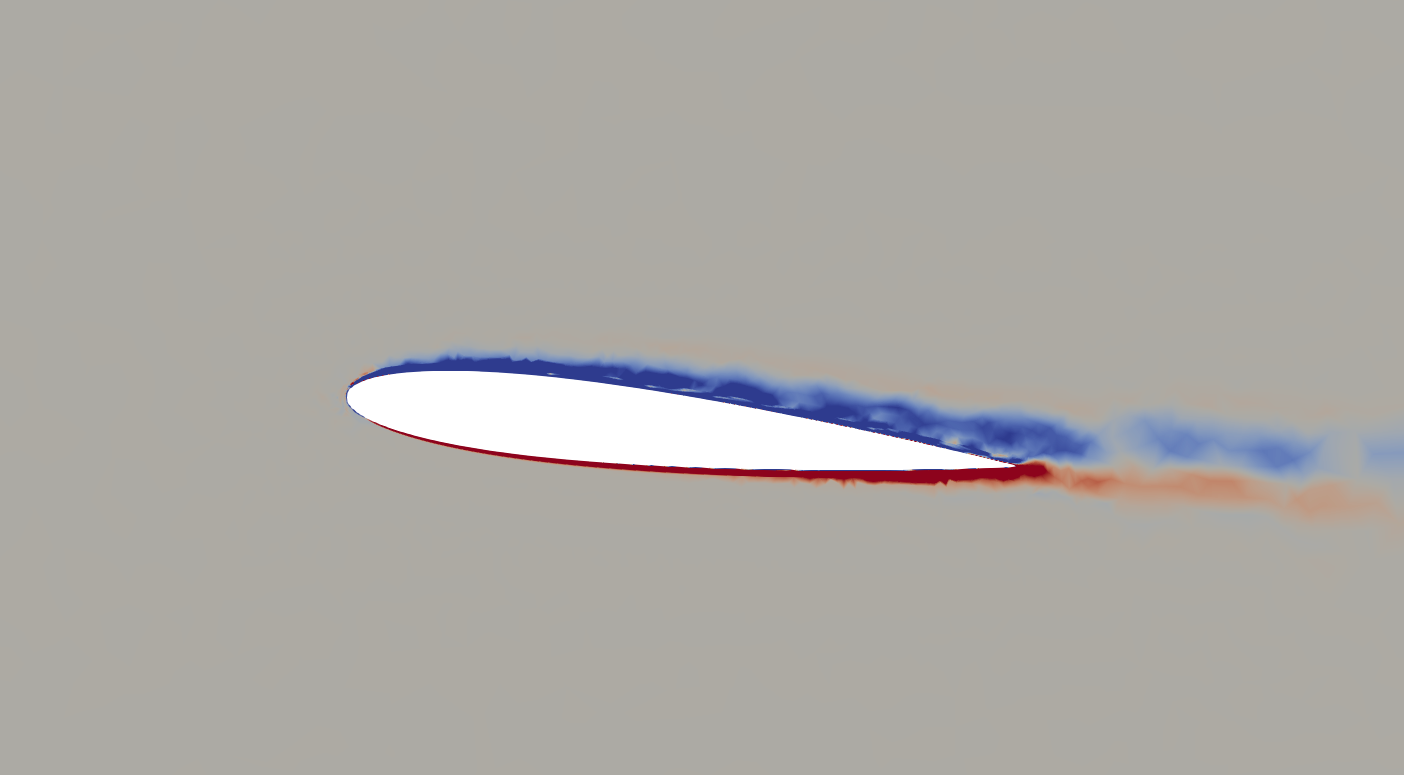
\includegraphics[width=1\textwidth]{figures/zonal_adapt_results/vorticity_plots_Re200k/M0/phase_210.png}
			\caption{M0 mesh, $\psi$ = $210^\circ$}
			\label{fig:M0_Re200k_sp_psi210}
		\end{subfigure}
	\end{center}
	\begin{subfigure}[b]{0.475\textwidth}
		\centering
		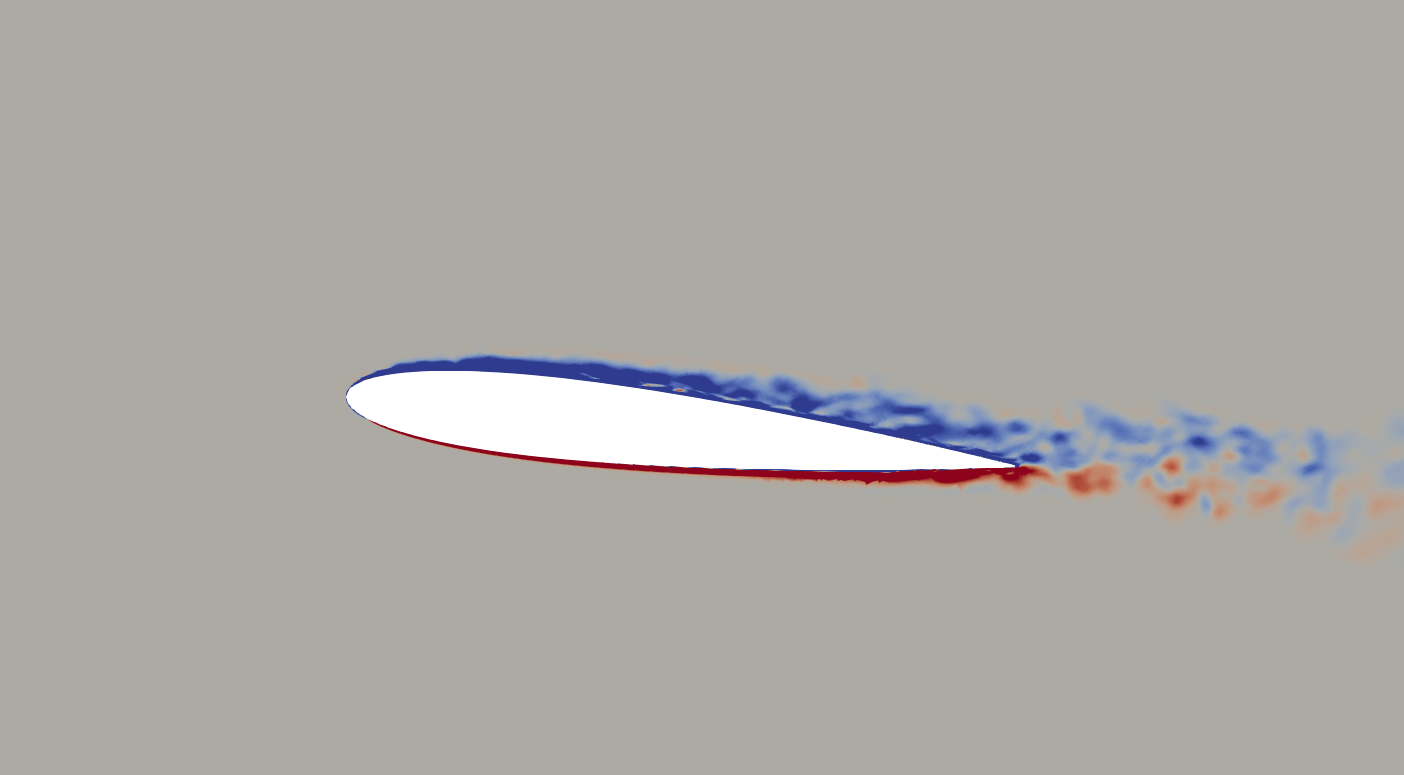
\includegraphics[width=1\textwidth]{figures/zonal_adapt_results/vorticity_plots_Re200k/Mza1_50/phase_210.png}
		\caption{Mza1\_25 mesh, $\psi$ = $210^\circ$}
		\label{fig:Mza1_50_Re200k_sp_psi210}
	\end{subfigure}
	\begin{subfigure}[b]{0.475\textwidth}
		\centering
		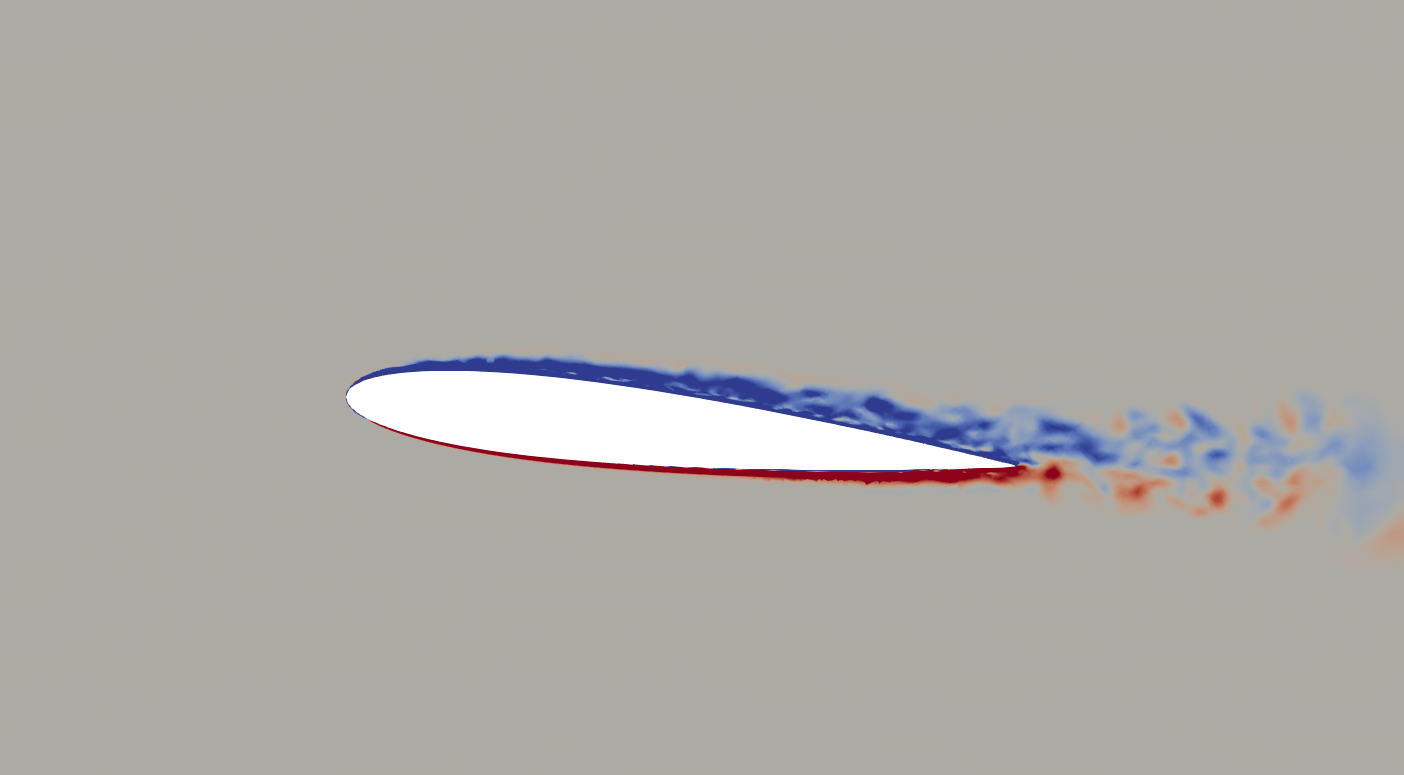
\includegraphics[width=1\textwidth]{figures/zonal_adapt_results/vorticity_plots_Re200k/Mza1_100/phase_210.png}
		\caption{Mza1\_100 mesh, $\psi$ = $210^\circ$}
		\label{fig:Mza1_100_Re200k_sp_psi210}
	\end{subfigure}
	%	\begin{subfigure}[b]{0.475\textwidth}
		%		\centering
		%		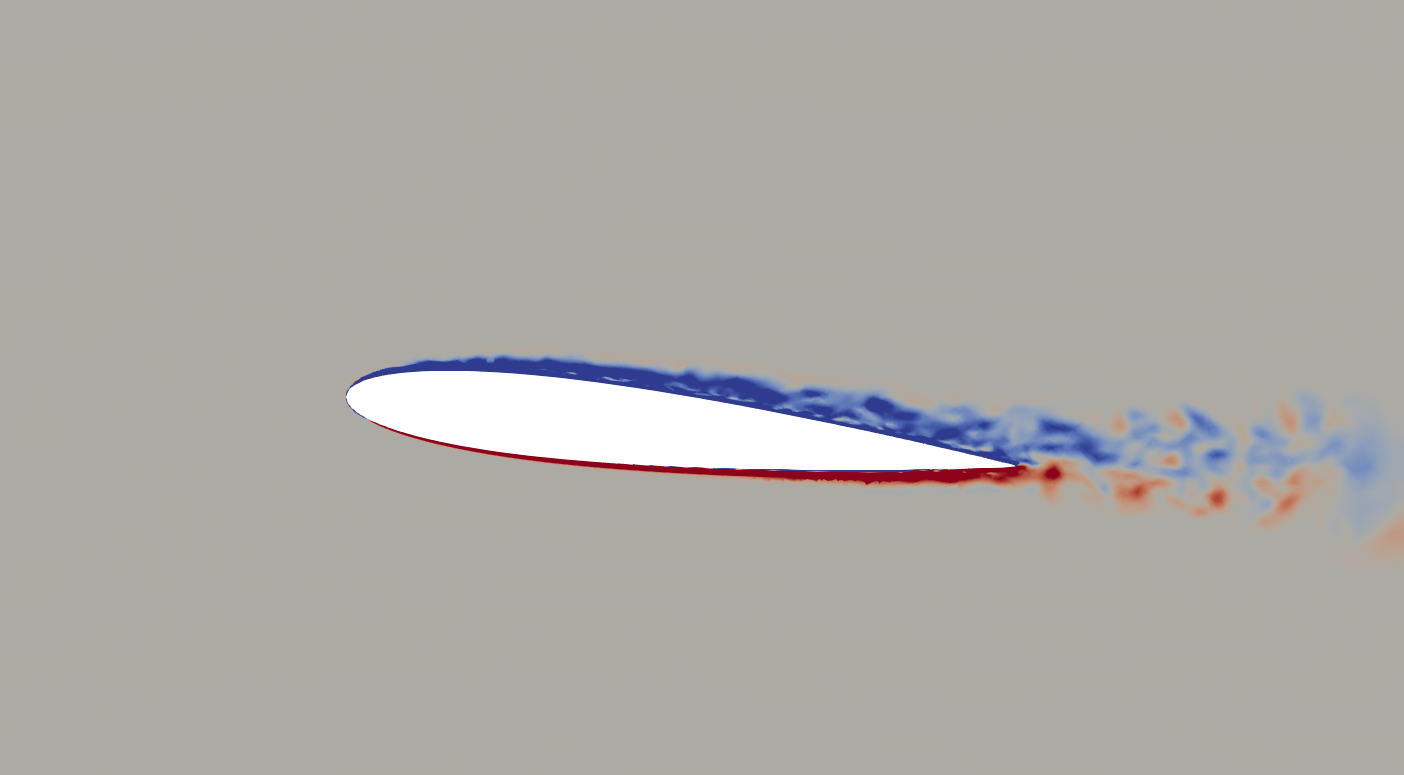
\includegraphics[width=1\textwidth]{figures/zonal_adapt_results/vorticity_plots_Re200k/Mza1_100/phase_210.png}
		%		\caption{Mza1\_100 mesh, $\psi$ = $210^\circ$}
		%		\label{fig:Mza1_100_Re200k_sp_psi210}
		%	\end{subfigure}
	%	\begin{subfigure}[b]{0.475\textwidth}
		%	\centering
		%	\includegraphics[width=1\textwidth]{figures/zonal_adapt_results/vorticity_plots_Re200k/Mza2_25/phase_210.png}
		%	\caption{Mza2\_25 mesh, $\psi$ = $210^\circ$}
		%	\label{fig:Mza2_25_Re200k_sp_psi210}
		%	\end{subfigure}
	\begin{subfigure}[b]{0.475\textwidth}
		\centering
		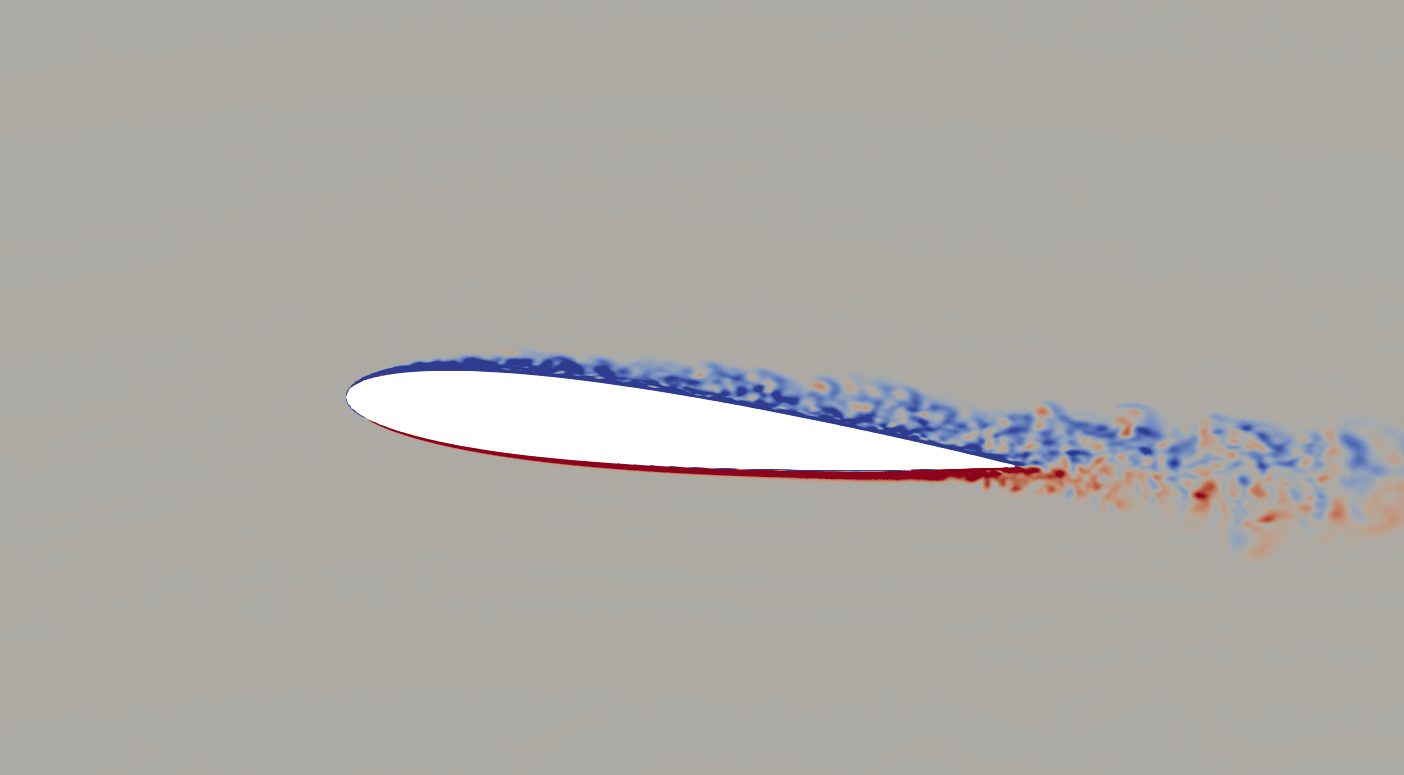
\includegraphics[width=1\textwidth]{figures/zonal_adapt_results/vorticity_plots_Re200k/Mza2_50/phase_210.png}
		\caption{Mza2\_50 mesh, $\psi$ = $210^\circ$}
		\label{fig:Mza2_50_Re200k_sp_psi210}
	\end{subfigure}	
	%	\begin{subfigure}[b]{0.475\textwidth}
		%		\centering
		%		\includegraphics[width=1\textwidth]{figures/zonal_adapt_results/vorticity_plots_Re200k/Mza2_100/phase_210.png}
		%		\caption{Mza2\_100 mesh, $\psi$ = $210^\circ$}
		%		\label{fig:Mza2_100_Re200k_sp_psi210}
		%	\end{subfigure}
	%	\begin{subfigure}[b]{0.475\textwidth}
		%	\centering
		%	\includegraphics[width=1\textwidth]{figures/zonal_adapt_results/vorticity_plots_Re200k/Mza3_50/phase_210.png}
		%	\caption{Mza3\_50 mesh, $\psi$ = $210^\circ$}
		%	\label{fig:Mza3_100_Re200k_sp_psi210}
		%	\end{subfigure}
	%	\begin{subfigure}[b]{0.475\textwidth}
		%		\centering
		%		\includegraphics[width=1\textwidth]{figures/zonal_adapt_results/vorticity_plots_Re200k/Mza3_100/phase_210.png}
		%		\caption{Mza3\_100 mesh, $\psi$ = $210^\circ$}
		%		\label{fig:Mza3_100_Re200k_sp_psi210}
		%	\end{subfigure}
	\caption{Spanwise vorticity comparison at $\psi$ = $210^\circ$ for different meshes}
	\label{fig:vorticity_Re200k_sp_210}
\end{figure}



%%=====================================
%% Phase = 240
%%=====================================


\begin{figure}[H]
	\centering
	\begin{center}
		\begin{subfigure}[b]{0.475\textwidth}
			\centering
			\includegraphics[width=1\textwidth]{figures/zonal_adapt_results/vorticity_plots_Re200k/M0/phase_240.png}
			\caption{M0 mesh, $\psi$ = $240^\circ$}
			\label{fig:M0_Re200k_sp_psi240}
		\end{subfigure}
	\end{center}
	\begin{subfigure}[b]{0.475\textwidth}
		\centering
		\includegraphics[width=1\textwidth]{figures/zonal_adapt_results/vorticity_plots_Re200k/Mza1_50/phase_240.png}
		\caption{Mza1\_25 mesh, $\psi$ = $240^\circ$}
		\label{fig:Mza1_50_Re200k_sp_psi240}
	\end{subfigure}
	\begin{subfigure}[b]{0.475\textwidth}
		\centering
		\includegraphics[width=1\textwidth]{figures/zonal_adapt_results/vorticity_plots_Re200k/Mza1_100/phase_240.png}
		\caption{Mza1\_100 mesh, $\psi$ = $240^\circ$}
		\label{fig:Mza1_100_Re200k_sp_psi240}
	\end{subfigure}
	%	\begin{subfigure}[b]{0.475\textwidth}
		%		\centering
		%		\includegraphics[width=1\textwidth]{figures/zonal_adapt_results/vorticity_plots_Re200k/Mza1_100/phase_240.png}
		%		\caption{Mza1\_100 mesh, $\psi$ = $240^\circ$}
		%		\label{fig:Mza1_100_Re200k_sp_psi240}
		%	\end{subfigure}
	%	\begin{subfigure}[b]{0.475\textwidth}
		%	\centering
		%	\includegraphics[width=1\textwidth]{figures/zonal_adapt_results/vorticity_plots_Re200k/Mza2_25/phase_240.png}
		%	\caption{Mza2\_25 mesh, $\psi$ = $240^\circ$}
		%	\label{fig:Mza2_25_Re200k_sp_psi240}
		%	\end{subfigure}
	\begin{subfigure}[b]{0.475\textwidth}
		\centering
		\includegraphics[width=1\textwidth]{figures/zonal_adapt_results/vorticity_plots_Re200k/Mza2_50/phase_240.png}
		\caption{Mza2\_50 mesh, $\psi$ = $240^\circ$}
		\label{fig:Mza2_50_Re200k_sp_psi240}
	\end{subfigure}	
	%	\begin{subfigure}[b]{0.475\textwidth}
		%		\centering
		%		\includegraphics[width=1\textwidth]{figures/zonal_adapt_results/vorticity_plots_Re200k/Mza2_100/phase_240.png}
		%		\caption{Mza2\_100 mesh, $\psi$ = $240^\circ$}
		%		\label{fig:Mza2_100_Re200k_sp_psi240}
		%	\end{subfigure}
	%	\begin{subfigure}[b]{0.475\textwidth}
		%	\centering
		%	\includegraphics[width=1\textwidth]{figures/zonal_adapt_results/vorticity_plots_Re200k/Mza3_50/phase_240.png}
		%	\caption{Mza3\_50 mesh, $\psi$ = $240^\circ$}
		%	\label{fig:Mza3_100_Re200k_sp_psi240}
		%	\end{subfigure}
	%	\begin{subfigure}[b]{0.475\textwidth}
		%		\centering
		%		\includegraphics[width=1\textwidth]{figures/zonal_adapt_results/vorticity_plots_Re200k/Mza3_100/phase_240.png}
		%		\caption{Mza3\_100 mesh, $\psi$ = $240^\circ$}
		%		\label{fig:Mza3_100_Re200k_sp_psi240}
		%	\end{subfigure}
	\caption{Spanwise vorticity comparison at $\psi$ = $240^\circ$ for different meshes}
	\label{fig:vorticity_Re200k_sp_240}
\end{figure}

%%=====================================
%% Phase = 255
%%=====================================

%\begin{figure}[H]
%	\centering
%	\begin{center}
%		\begin{subfigure}[b]{0.475\textwidth}
%			\centering
%			\includegraphics[width=1\textwidth]{figures/zonal_adapt_results/vorticity_plots_Re200k/M0/phase_255.png}
%			\caption{M0 mesh, $\psi$ = $255^\circ$}
%			\label{fig:M0_Re200k_sp_psi255}
%		\end{subfigure}
%	\end{center}
%	\begin{subfigure}[b]{0.475\textwidth}
%		\centering
%		\includegraphics[width=1\textwidth]{figures/zonal_adapt_results/vorticity_plots_Re200k/Mza1_50/phase_255.png}
%		\caption{Mza1\_25 mesh, $\psi$ = $255^\circ$}
%		\label{fig:Mza1_50_Re200k_sp_psi255}
%	\end{subfigure}
%	\begin{subfigure}[b]{0.475\textwidth}
%		\centering
%		\includegraphics[width=1\textwidth]{figures/zonal_adapt_results/vorticity_plots_Re200k/Mza1_100/phase_255.png}
%		\caption{Mza1\_100 mesh, $\psi$ = $255^\circ$}
%		\label{fig:Mza1_100_Re200k_sp_psi255}
%	\end{subfigure}
%	%	\begin{subfigure}[b]{0.475\textwidth}
%		%		\centering
%		%		\includegraphics[width=1\textwidth]{figures/zonal_adapt_results/vorticity_plots_Re200k/Mza1_100/phase_255.png}
%		%		\caption{Mza1\_100 mesh, $\psi$ = $255^\circ$}
%		%		\label{fig:Mza1_100_Re200k_sp_psi255}
%		%	\end{subfigure}
%	%	\begin{subfigure}[b]{0.475\textwidth}
%		%	\centering
%		%	\includegraphics[width=1\textwidth]{figures/zonal_adapt_results/vorticity_plots_Re200k/Mza2_25/phase_255.png}
%		%	\caption{Mza2\_25 mesh, $\psi$ = $255^\circ$}
%		%	\label{fig:Mza2_25_Re200k_sp_psi255}
%		%	\end{subfigure}
%	\begin{subfigure}[b]{0.475\textwidth}
%		\centering
%		\includegraphics[width=1\textwidth]{figures/zonal_adapt_results/vorticity_plots_Re200k/Mza2_50/phase_255.png}
%		\caption{Mza2\_50 mesh, $\psi$ = $255^\circ$}
%		\label{fig:Mza2_50_Re200k_sp_psi255}
%	\end{subfigure}	
%	%	\begin{subfigure}[b]{0.475\textwidth}
%		%		\centering
%		%		\includegraphics[width=1\textwidth]{figures/zonal_adapt_results/vorticity_plots_Re200k/Mza2_100/phase_255.png}
%		%		\caption{Mza2\_100 mesh, $\psi$ = $255^\circ$}
%		%		\label{fig:Mza2_100_Re200k_sp_psi255}
%		%	\end{subfigure}
%	%	\begin{subfigure}[b]{0.475\textwidth}
%		%	\centering
%		%	\includegraphics[width=1\textwidth]{figures/zonal_adapt_results/vorticity_plots_Re200k/Mza3_50/phase_255.png}
%		%	\caption{Mza3\_50 mesh, $\psi$ = $255^\circ$}
%		%	\label{fig:Mza3_100_Re200k_sp_psi255}
%		%	\end{subfigure}
%	%	\begin{subfigure}[b]{0.475\textwidth}
%		%		\centering
%		%		\includegraphics[width=1\textwidth]{figures/zonal_adapt_results/vorticity_plots_Re200k/Mza3_100/phase_255.png}
%		%		\caption{Mza3\_100 mesh, $\psi$ = $255^\circ$}
%		%		\label{fig:Mza3_100_Re200k_sp_psi255}
%		%	\end{subfigure}
%	\caption{Spanwise vorticity comparison at $\psi$ = $255^\circ$ for different meshes}
%	\label{fig:vorticity_Re200k_sp_255}
%\end{figure}




%%=====================================
%% Phase = 270
%%=====================================

\begin{figure}[H]
	\centering
	\begin{center}
		\begin{subfigure}[b]{0.475\textwidth}
			\centering
			\includegraphics[width=1\textwidth]{figures/zonal_adapt_results/vorticity_plots_Re200k/M0/phase_270.png}
			\caption{M0 mesh, $\psi$ = $270^\circ$}
			\label{fig:M0_Re200k_sp_psi270}
		\end{subfigure}
	\end{center}
	\begin{subfigure}[b]{0.475\textwidth}
		\centering
		\includegraphics[width=1\textwidth]{figures/zonal_adapt_results/vorticity_plots_Re200k/Mza1_50/phase_270.png}
		\caption{Mza1\_25 mesh, $\psi$ = $270^\circ$}
		\label{fig:Mza1_50_Re200k_sp_psi270}
	\end{subfigure}
	\begin{subfigure}[b]{0.475\textwidth}
		\centering
		\includegraphics[width=1\textwidth]{figures/zonal_adapt_results/vorticity_plots_Re200k/Mza1_100/phase_270.png}
		\caption{Mza1\_100 mesh, $\psi$ = $270^\circ$}
		\label{fig:Mza1_100_Re200k_sp_psi270}
	\end{subfigure}
	%	\begin{subfigure}[b]{0.475\textwidth}
		%		\centering
		%		\includegraphics[width=1\textwidth]{figures/zonal_adapt_results/vorticity_plots_Re200k/Mza1_100/phase_270.png}
		%		\caption{Mza1\_100 mesh, $\psi$ = $270^\circ$}
		%		\label{fig:Mza1_100_Re200k_sp_psi270}
		%	\end{subfigure}
	%	\begin{subfigure}[b]{0.475\textwidth}
		%	\centering
		%	\includegraphics[width=1\textwidth]{figures/zonal_adapt_results/vorticity_plots_Re200k/Mza2_25/phase_270.png}
		%	\caption{Mza2\_25 mesh, $\psi$ = $270^\circ$}
		%	\label{fig:Mza2_25_Re200k_sp_psi270}
		%	\end{subfigure}
	\begin{subfigure}[b]{0.475\textwidth}
		\centering
		\includegraphics[width=1\textwidth]{figures/zonal_adapt_results/vorticity_plots_Re200k/Mza2_50/phase_270.png}
		\caption{Mza2\_50 mesh, $\psi$ = $270^\circ$}
		\label{fig:Mza2_50_Re200k_sp_psi270}
	\end{subfigure}	
	%	\begin{subfigure}[b]{0.475\textwidth}
		%		\centering
		%		\includegraphics[width=1\textwidth]{figures/zonal_adapt_results/vorticity_plots_Re200k/Mza2_100/phase_270.png}
		%		\caption{Mza2\_100 mesh, $\psi$ = $270^\circ$}
		%		\label{fig:Mza2_100_Re200k_sp_psi270}
		%	\end{subfigure}
	%	\begin{subfigure}[b]{0.475\textwidth}
		%	\centering
		%	\includegraphics[width=1\textwidth]{figures/zonal_adapt_results/vorticity_plots_Re200k/Mza3_50/phase_270.png}
		%	\caption{Mza3\_50 mesh, $\psi$ = $270^\circ$}
		%	\label{fig:Mza3_100_Re200k_sp_psi270}
		%	\end{subfigure}
	%	\begin{subfigure}[b]{0.475\textwidth}
		%		\centering
		%		\includegraphics[width=1\textwidth]{figures/zonal_adapt_results/vorticity_plots_Re200k/Mza3_100/phase_270.png}
		%		\caption{Mza3\_100 mesh, $\psi$ = $270^\circ$}
		%		\label{fig:Mza3_100_Re200k_sp_psi270}
		%	\end{subfigure}
	\caption{Spanwise vorticity comparison at $\psi$ = $270^\circ$ for different meshes}
	\label{fig:vorticity_Re200k_sp_270}
\end{figure}

%%=====================================
%% Phase = 285
%%=====================================

%\begin{figure}[H]
%	\centering
%	\begin{center}
%		\begin{subfigure}[b]{0.475\textwidth}
%			\centering
%			\includegraphics[width=1\textwidth]{figures/zonal_adapt_results/vorticity_plots_Re200k/M0/phase_285.png}
%			\caption{M0 mesh, $\psi$ = $285^\circ$}
%			\label{fig:M0_Re200k_sp_psi285}
%		\end{subfigure}
%	\end{center}
%	\begin{subfigure}[b]{0.475\textwidth}
%		\centering
%		\includegraphics[width=1\textwidth]{figures/zonal_adapt_results/vorticity_plots_Re200k/Mza1_50/phase_285.png}
%		\caption{Mza1\_25 mesh, $\psi$ = $285^\circ$}
%		\label{fig:Mza1_50_Re200k_sp_psi285}
%	\end{subfigure}
%	\begin{subfigure}[b]{0.475\textwidth}
%		\centering
%		\includegraphics[width=1\textwidth]{figures/zonal_adapt_results/vorticity_plots_Re200k/Mza1_100/phase_285.png}
%		\caption{Mza1\_100 mesh, $\psi$ = $285^\circ$}
%		\label{fig:Mza1_100_Re200k_sp_psi285}
%	\end{subfigure}
%	%	\begin{subfigure}[b]{0.475\textwidth}
%		%		\centering
%		%		\includegraphics[width=1\textwidth]{figures/zonal_adapt_results/vorticity_plots_Re200k/Mza1_100/phase_285.png}
%		%		\caption{Mza1\_100 mesh, $\psi$ = $285^\circ$}
%		%		\label{fig:Mza1_100_Re200k_sp_psi285}
%		%	\end{subfigure}
%	%	\begin{subfigure}[b]{0.475\textwidth}
%		%	\centering
%		%	\includegraphics[width=1\textwidth]{figures/zonal_adapt_results/vorticity_plots_Re200k/Mza2_25/phase_285.png}
%		%	\caption{Mza2\_25 mesh, $\psi$ = $285^\circ$}
%		%	\label{fig:Mza2_25_Re200k_sp_psi285}
%		%	\end{subfigure}
%	\begin{subfigure}[b]{0.475\textwidth}
%		\centering
%		\includegraphics[width=1\textwidth]{figures/zonal_adapt_results/vorticity_plots_Re200k/Mza2_50/phase_285.png}
%		\caption{Mza2\_50 mesh, $\psi$ = $285^\circ$}
%		\label{fig:Mza2_50_Re200k_sp_psi285}
%	\end{subfigure}	
%	%	\begin{subfigure}[b]{0.475\textwidth}
%		%		\centering
%		%		\includegraphics[width=1\textwidth]{figures/zonal_adapt_results/vorticity_plots_Re200k/Mza2_100/phase_285.png}
%		%		\caption{Mza2\_100 mesh, $\psi$ = $285^\circ$}
%		%		\label{fig:Mza2_100_Re200k_sp_psi285}
%		%	\end{subfigure}
%	%	\begin{subfigure}[b]{0.475\textwidth}
%		%	\centering
%		%	\includegraphics[width=1\textwidth]{figures/zonal_adapt_results/vorticity_plots_Re200k/Mza3_50/phase_285.png}
%		%	\caption{Mza3\_50 mesh, $\psi$ = $285^\circ$}
%		%	\label{fig:Mza3_100_Re200k_sp_psi285}
%		%	\end{subfigure}
%	%	\begin{subfigure}[b]{0.475\textwidth}
%		%		\centering
%		%		\includegraphics[width=1\textwidth]{figures/zonal_adapt_results/vorticity_plots_Re200k/Mza3_100/phase_285.png}
%		%		\caption{Mza3\_100 mesh, $\psi$ = $285^\circ$}
%		%		\label{fig:Mza3_100_Re200k_sp_psi285}
%		%	\end{subfigure}
%	\caption{Spanwise vorticity comparison at $\psi$ = $285^\circ$ for different meshes}
%	\label{fig:vorticity_Re200k_sp_285}
%\end{figure}


%%=====================================
%% Phase = 300
%%=====================================

\begin{figure}[H]
	\centering
	\begin{center}
		\begin{subfigure}[b]{0.475\textwidth}
			\centering
			\includegraphics[width=1\textwidth]{figures/zonal_adapt_results/vorticity_plots_Re200k/M0/phase_300.png}
			\caption{M0 mesh, $\psi$ = $300^\circ$}
			\label{fig:M0_Re200k_sp_psi300}
		\end{subfigure}
	\end{center}
	\begin{subfigure}[b]{0.475\textwidth}
		\centering
		\includegraphics[width=1\textwidth]{figures/zonal_adapt_results/vorticity_plots_Re200k/Mza1_50/phase_300.png}
		\caption{Mza1\_25 mesh, $\psi$ = $300^\circ$}
		\label{fig:Mza1_50_Re200k_sp_psi300}
	\end{subfigure}
	\begin{subfigure}[b]{0.475\textwidth}
		\centering
		\includegraphics[width=1\textwidth]{figures/zonal_adapt_results/vorticity_plots_Re200k/Mza1_100/phase_300.png}
		\caption{Mza1\_100 mesh, $\psi$ = $300^\circ$}
		\label{fig:Mza1_100_Re200k_sp_psi300}
	\end{subfigure}
	%	\begin{subfigure}[b]{0.475\textwidth}
		%		\centering
		%		\includegraphics[width=1\textwidth]{figures/zonal_adapt_results/vorticity_plots_Re200k/Mza1_100/phase_300.png}
		%		\caption{Mza1\_100 mesh, $\psi$ = $300^\circ$}
		%		\label{fig:Mza1_100_Re200k_sp_psi300}
		%	\end{subfigure}
	%	\begin{subfigure}[b]{0.475\textwidth}
		%	\centering
		%	\includegraphics[width=1\textwidth]{figures/zonal_adapt_results/vorticity_plots_Re200k/Mza2_25/phase_300.png}
		%	\caption{Mza2\_25 mesh, $\psi$ = $300^\circ$}
		%	\label{fig:Mza2_25_Re200k_sp_psi300}
		%	\end{subfigure}
	\begin{subfigure}[b]{0.475\textwidth}
		\centering
		\includegraphics[width=1\textwidth]{figures/zonal_adapt_results/vorticity_plots_Re200k/Mza2_50/phase_300.png}
		\caption{Mza2\_50 mesh, $\psi$ = $300^\circ$}
		\label{fig:Mza2_50_Re200k_sp_psi300}
	\end{subfigure}	
	%	\begin{subfigure}[b]{0.475\textwidth}
		%		\centering
		%		\includegraphics[width=1\textwidth]{figures/zonal_adapt_results/vorticity_plots_Re200k/Mza2_100/phase_300.png}
		%		\caption{Mza2\_100 mesh, $\psi$ = $300^\circ$}
		%		\label{fig:Mza2_100_Re200k_sp_psi300}
		%	\end{subfigure}
	%	\begin{subfigure}[b]{0.475\textwidth}
		%	\centering
		%	\includegraphics[width=1\textwidth]{figures/zonal_adapt_results/vorticity_plots_Re200k/Mza3_50/phase_300.png}
		%	\caption{Mza3\_50 mesh, $\psi$ = $300^\circ$}
		%	\label{fig:Mza3_100_Re200k_sp_psi300}
		%	\end{subfigure}
	%	\begin{subfigure}[b]{0.475\textwidth}
		%		\centering
		%		\includegraphics[width=1\textwidth]{figures/zonal_adapt_results/vorticity_plots_Re200k/Mza3_100/phase_300.png}
		%		\caption{Mza3\_100 mesh, $\psi$ = $300^\circ$}
		%		\label{fig:Mza3_100_Re200k_sp_psi300}
		%	\end{subfigure}
	\caption{Spanwise vorticity comparison at $\psi$ = $300^\circ$ for different meshes}
	\label{fig:vorticity_Re200k_sp_300}
\end{figure}

%%=====================================
%% Phase = 315
%%=====================================

%\begin{figure}[H]
%	\centering
%	\begin{center}
%		\begin{subfigure}[b]{0.475\textwidth}
%			\centering
%			\includegraphics[width=1\textwidth]{figures/zonal_adapt_results/vorticity_plots_Re200k/M0/phase_315.png}
%			\caption{M0 mesh, $\psi$ = $315^\circ$}
%			\label{fig:M0_Re200k_sp_psi315}
%		\end{subfigure}
%	\end{center}
%	\begin{subfigure}[b]{0.475\textwidth}
%		\centering
%		\includegraphics[width=1\textwidth]{figures/zonal_adapt_results/vorticity_plots_Re200k/Mza1_50/phase_315.png}
%		\caption{Mza1\_25 mesh, $\psi$ = $315^\circ$}
%		\label{fig:Mza1_50_Re200k_sp_psi315}
%	\end{subfigure}
%	\begin{subfigure}[b]{0.475\textwidth}
%		\centering
%		\includegraphics[width=1\textwidth]{figures/zonal_adapt_results/vorticity_plots_Re200k/Mza1_100/phase_315.png}
%		\caption{Mza1\_100 mesh, $\psi$ = $315^\circ$}
%		\label{fig:Mza1_100_Re200k_sp_psi315}
%	\end{subfigure}
%	%	\begin{subfigure}[b]{0.475\textwidth}
%		%		\centering
%		%		\includegraphics[width=1\textwidth]{figures/zonal_adapt_results/vorticity_plots_Re200k/Mza1_100/phase_315.png}
%		%		\caption{Mza1\_100 mesh, $\psi$ = $315^\circ$}
%		%		\label{fig:Mza1_100_Re200k_sp_psi315}
%		%	\end{subfigure}
%	%	\begin{subfigure}[b]{0.475\textwidth}
%		%	\centering
%		%	\includegraphics[width=1\textwidth]{figures/zonal_adapt_results/vorticity_plots_Re200k/Mza2_25/phase_315.png}
%		%	\caption{Mza2\_25 mesh, $\psi$ = $315^\circ$}
%		%	\label{fig:Mza2_25_Re200k_sp_psi315}
%		%	\end{subfigure}
%	\begin{subfigure}[b]{0.475\textwidth}
%		\centering
%		\includegraphics[width=1\textwidth]{figures/zonal_adapt_results/vorticity_plots_Re200k/Mza2_50/phase_315.png}
%		\caption{Mza2\_50 mesh, $\psi$ = $315^\circ$}
%		\label{fig:Mza2_50_Re200k_sp_psi315}
%	\end{subfigure}	
%	%	\begin{subfigure}[b]{0.475\textwidth}
%		%		\centering
%		%		\includegraphics[width=1\textwidth]{figures/zonal_adapt_results/vorticity_plots_Re200k/Mza2_100/phase_315.png}
%		%		\caption{Mza2\_100 mesh, $\psi$ = $315^\circ$}
%		%		\label{fig:Mza2_100_Re200k_sp_psi315}
%		%	\end{subfigure}
%	%	\begin{subfigure}[b]{0.475\textwidth}
%		%	\centering
%		%	\includegraphics[width=1\textwidth]{figures/zonal_adapt_results/vorticity_plots_Re200k/Mza3_50/phase_315.png}
%		%	\caption{Mza3\_50 mesh, $\psi$ = $315^\circ$}
%		%	\label{fig:Mza3_100_Re200k_sp_psi315}
%		%	\end{subfigure}
%	%	\begin{subfigure}[b]{0.475\textwidth}
%		%		\centering
%		%		\includegraphics[width=1\textwidth]{figures/zonal_adapt_results/vorticity_plots_Re200k/Mza3_100/phase_315.png}
%		%		\caption{Mza3\_100 mesh, $\psi$ = $315^\circ$}
%		%		\label{fig:Mza3_100_Re200k_sp_psi315}
%		%	\end{subfigure}
%	\caption{Spanwise vorticity comparison at $\psi$ = $315^\circ$ for different meshes}
%	\label{fig:vorticity_Re200k_sp_315}
>>>>>>> 86e8ea47e8afdbcf5b6dcff28089dc063f35150b
%\end{figure}